%%%%%%%%%%%%%%%%%%%%%%%%%%%%%%%%%%
\section{Results with collinear photon-PDFs}
%%%%%%%%%%%%%%%%%%%%%%%%%%%%%%%%%%

We start with the calculation of the elastic contribution, $p+\textrm{Pb}\rightarrow p+\textrm{Pb}+ \ell^+\ell^-$.
In this case the photon flux becomes:
\begin{equation}
f_\gamma^{p}(x,\mu) = f_\gamma^{p}(x) 
\end{equation}
and the following parameterization is used~\cite{}:
\begin{equation}
f_\gamma^{p}(x) = \frac{\alpha}{\pi}
\left(
\frac{1-x+0.5x^2}{x}
\right)
\left(
\frac{A+3}{A-1}\log{A}-\frac{17}{6}-\frac{4}{3A}+\frac{1}{6A^2}
\right)~,
\end{equation}
where $A = 1+\frac{Q_0^2(1-x)}{x m_p^2}$ and $Q_0^2 = 0.71$~\GeV$^2$.

The results for the elastic case are cross-checked with the calculation from STARlight MC and a good agreement is found:
$\sigma_{fid}^{\textrm{el}} = 17.5$~nb, whereas $\sigma_{fid}^{\textrm{STARlight}} = 17.0$~nb.
Both calculations are also corrected by a factor $S^2=0.96$ which takes into account the requirement that there be no hadronic interactions between the proton and the ion. This is calculated using STARlight, where the hard-sphere proton--nucleus requirement~\cite{Klein:2016yzr} is used.

Next, for the inelastic case ($\gamma p\rightarrow \ell^+\ell^- + X$), several recent parameterizations of the photon parton distributions are studied: CT14qed~\cite{Schmidt:2015zda}, LUXqed17~\cite{Manohar:2017eqh} and NNPDF3.1luxQED~\cite{Bertone:2017bme}.
Comparison of several lepton kinematic distributions between different photon-PDFs are shown in Fig.~\ref{fig:elastic},\ref{fig:elastic_cut},\ref{fig:inc},\ref{fig:inc_cut}.

\begin{figure}[h!]
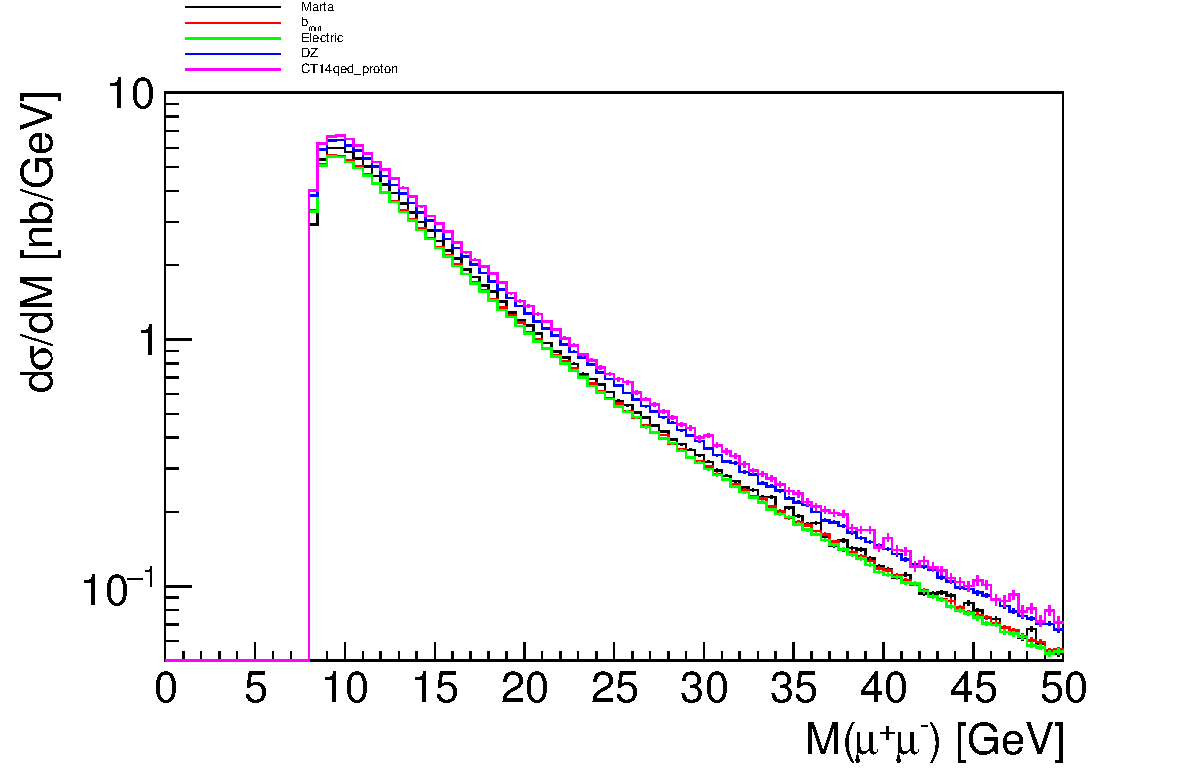
\includegraphics[width=0.4\textwidth]{figures/Mll_elastic.pdf}
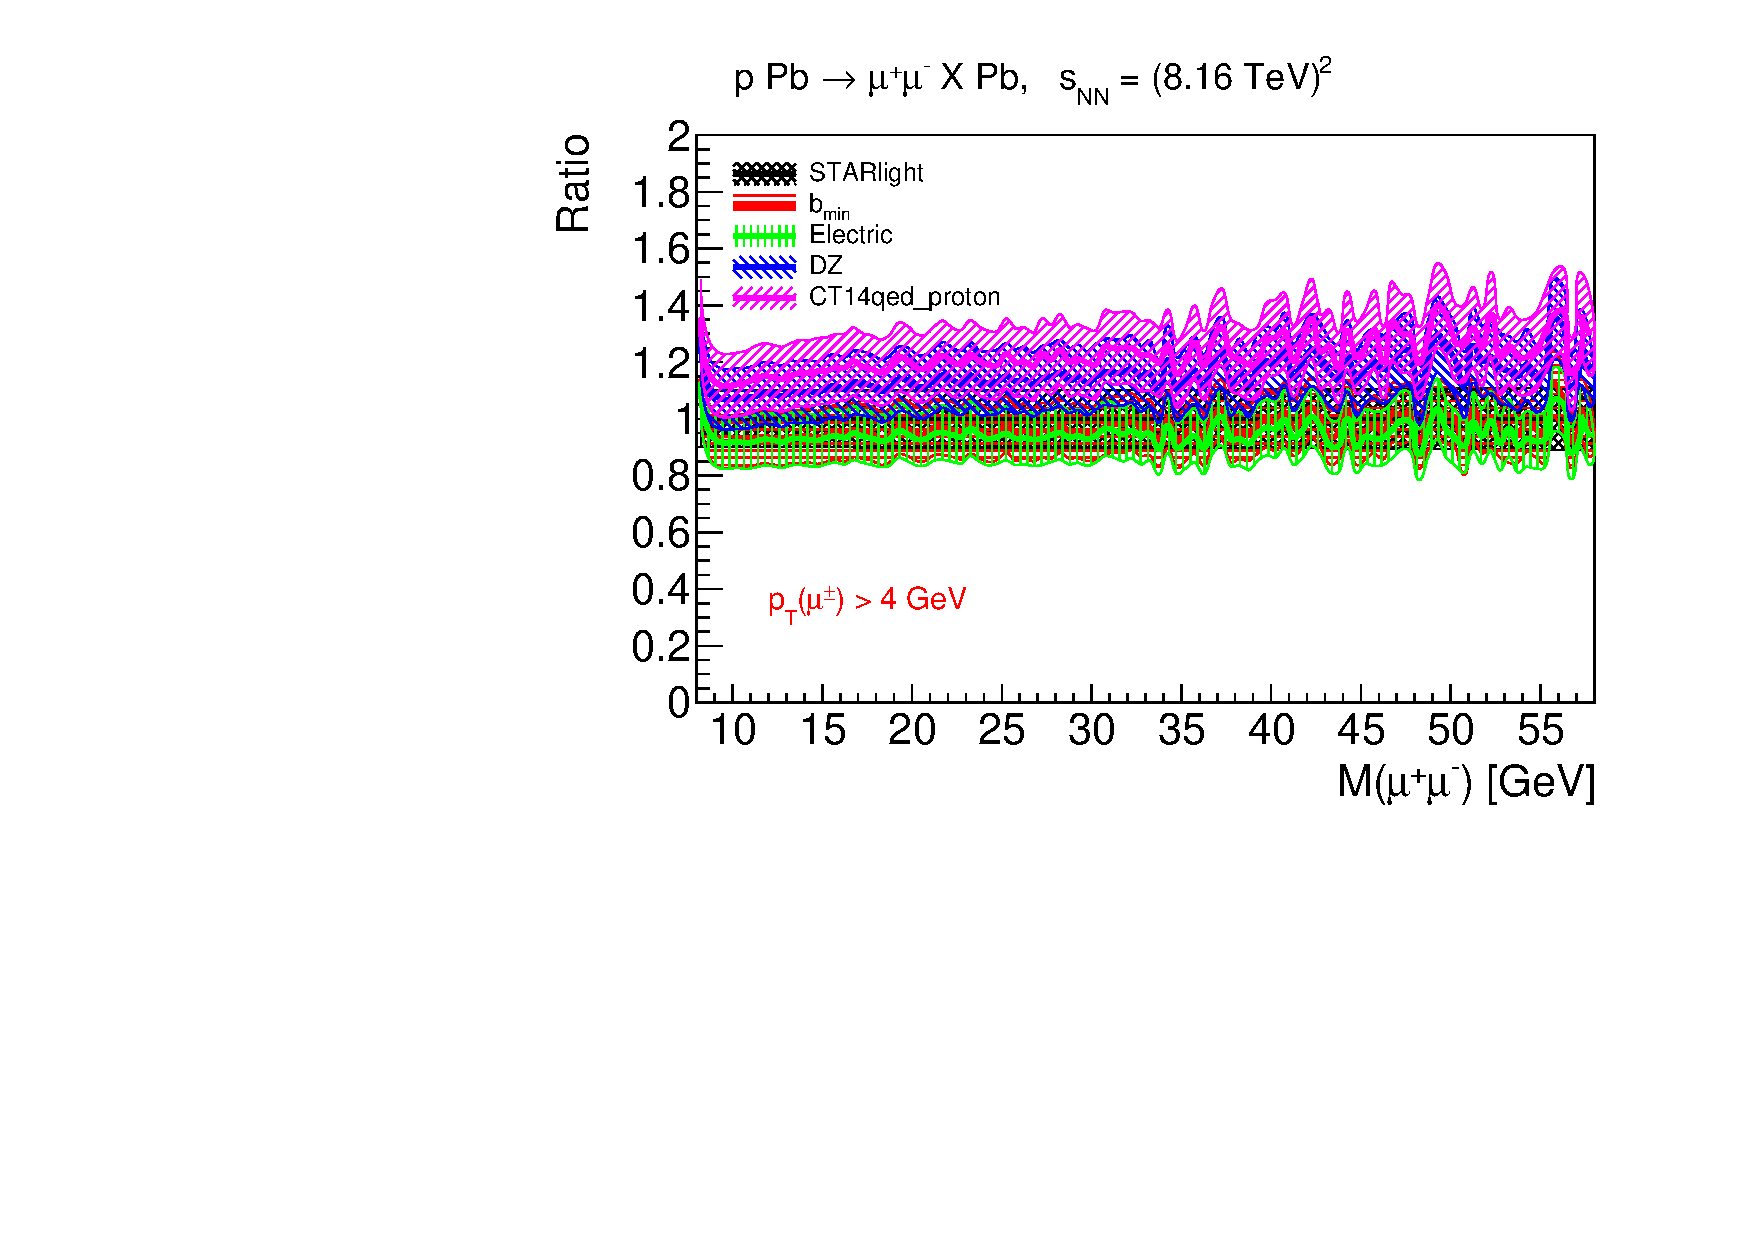
\includegraphics[width=0.4\textwidth]{figures/RatioMll_elastic.pdf}
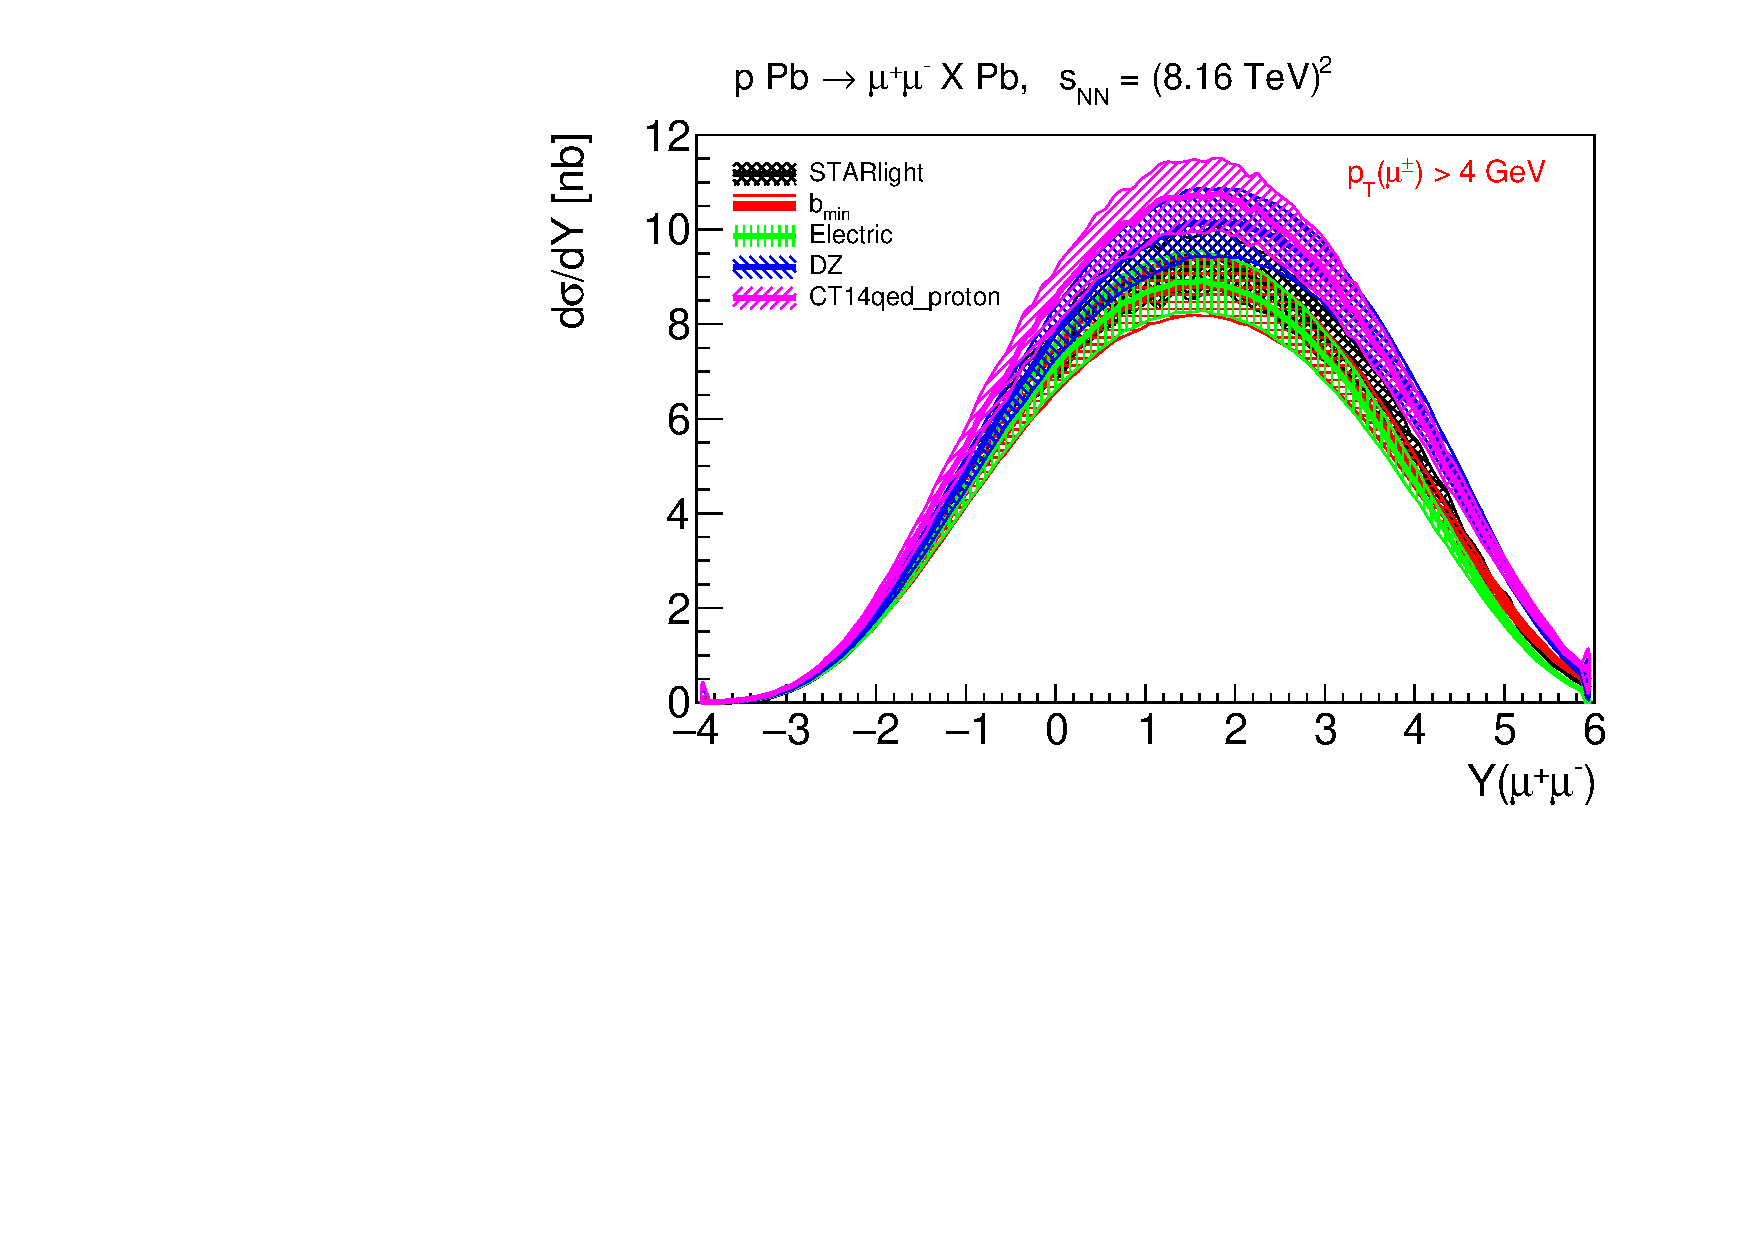
\includegraphics[width=0.4\textwidth]{figures/Yll_elastic.pdf}
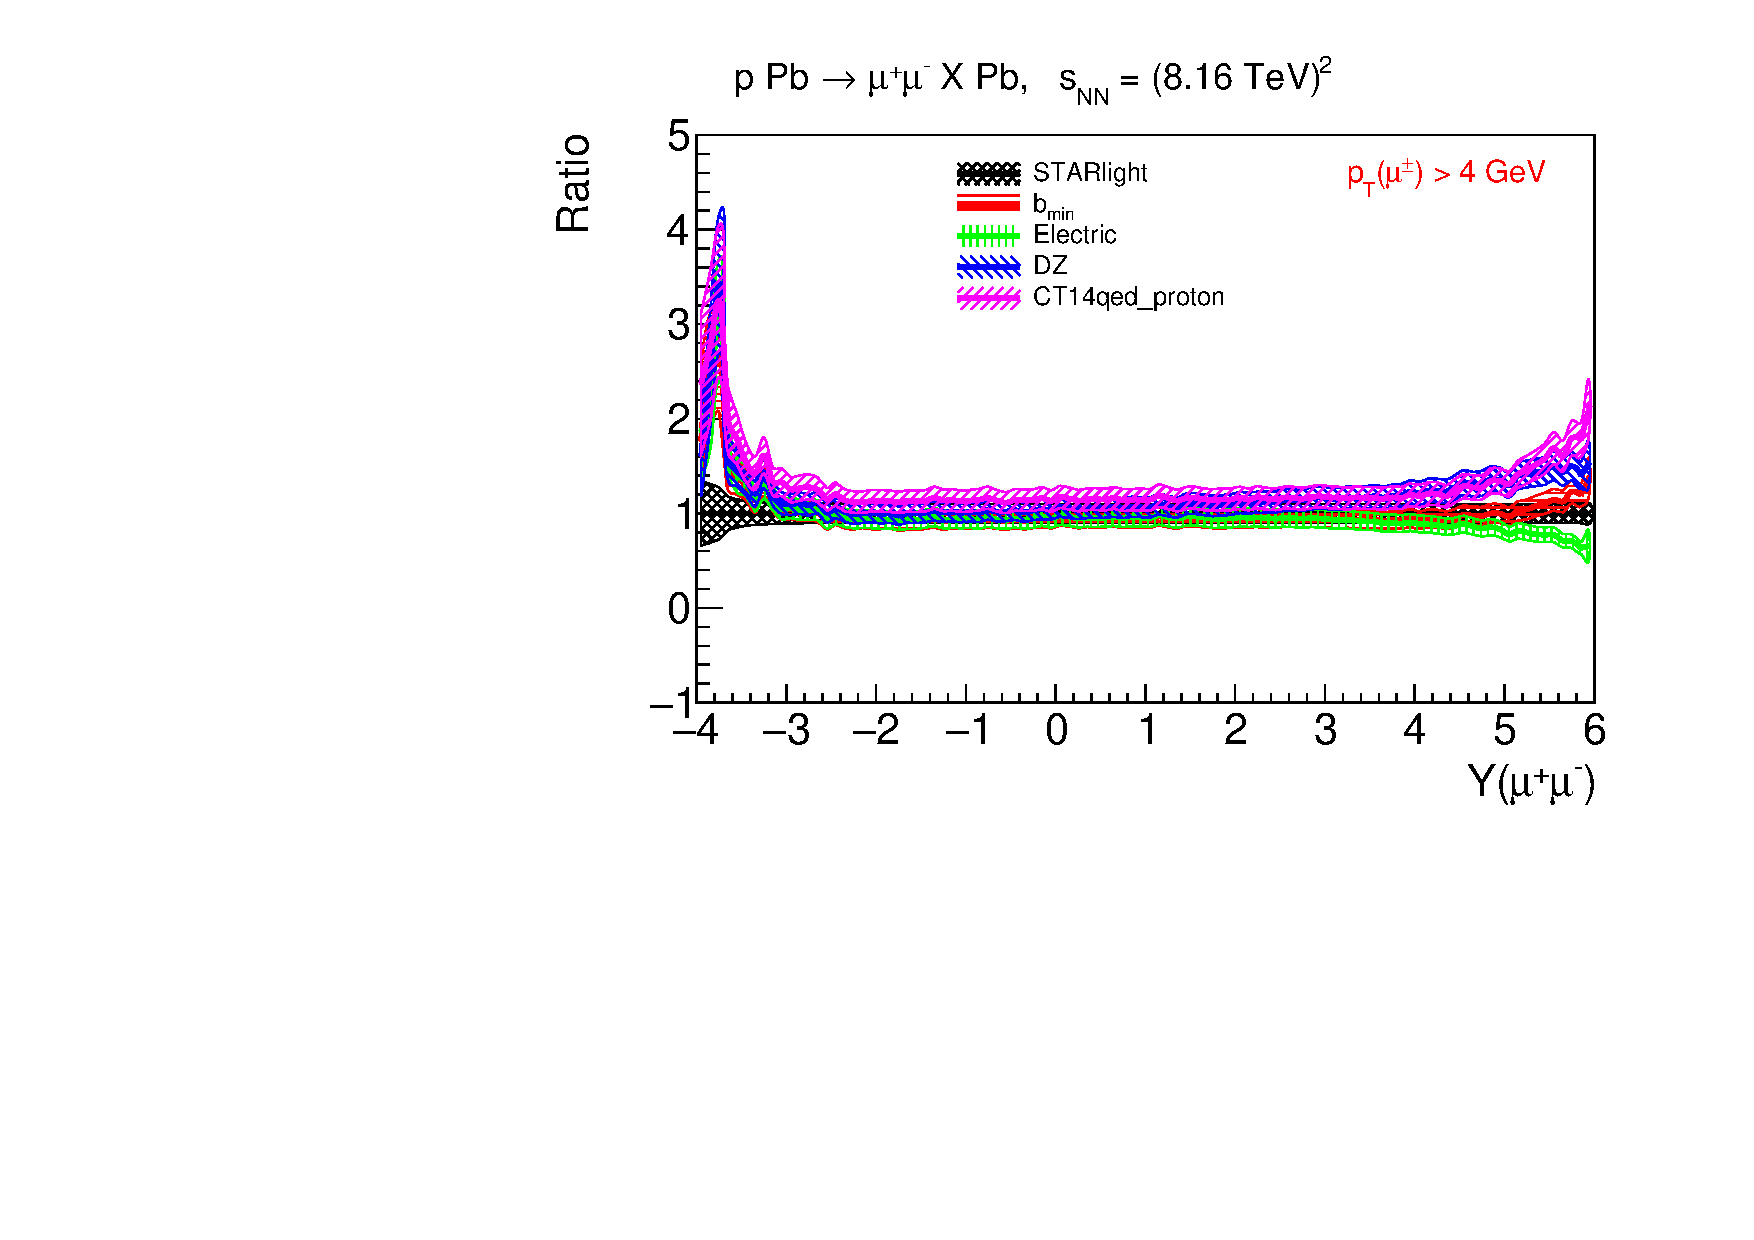
\includegraphics[width=0.4\textwidth]{figures/RatioYll_elastic.pdf}
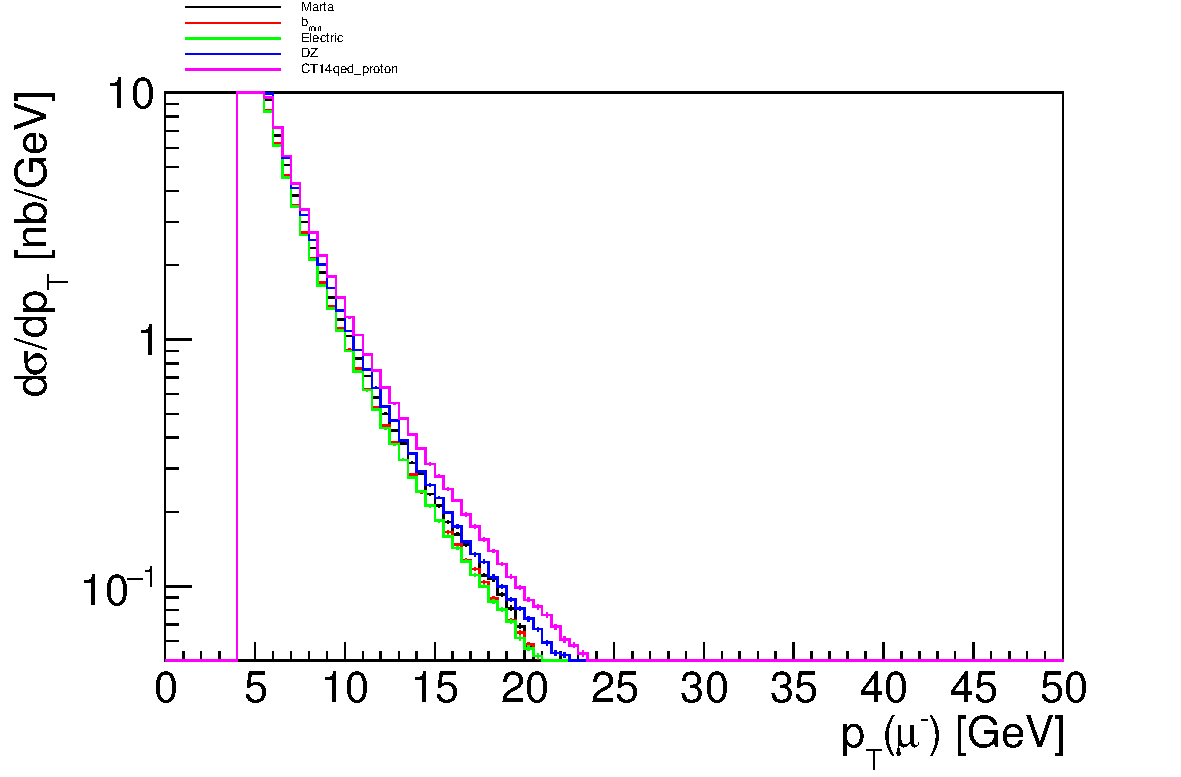
\includegraphics[width=0.4\textwidth]{figures/pTl_elastic.pdf}
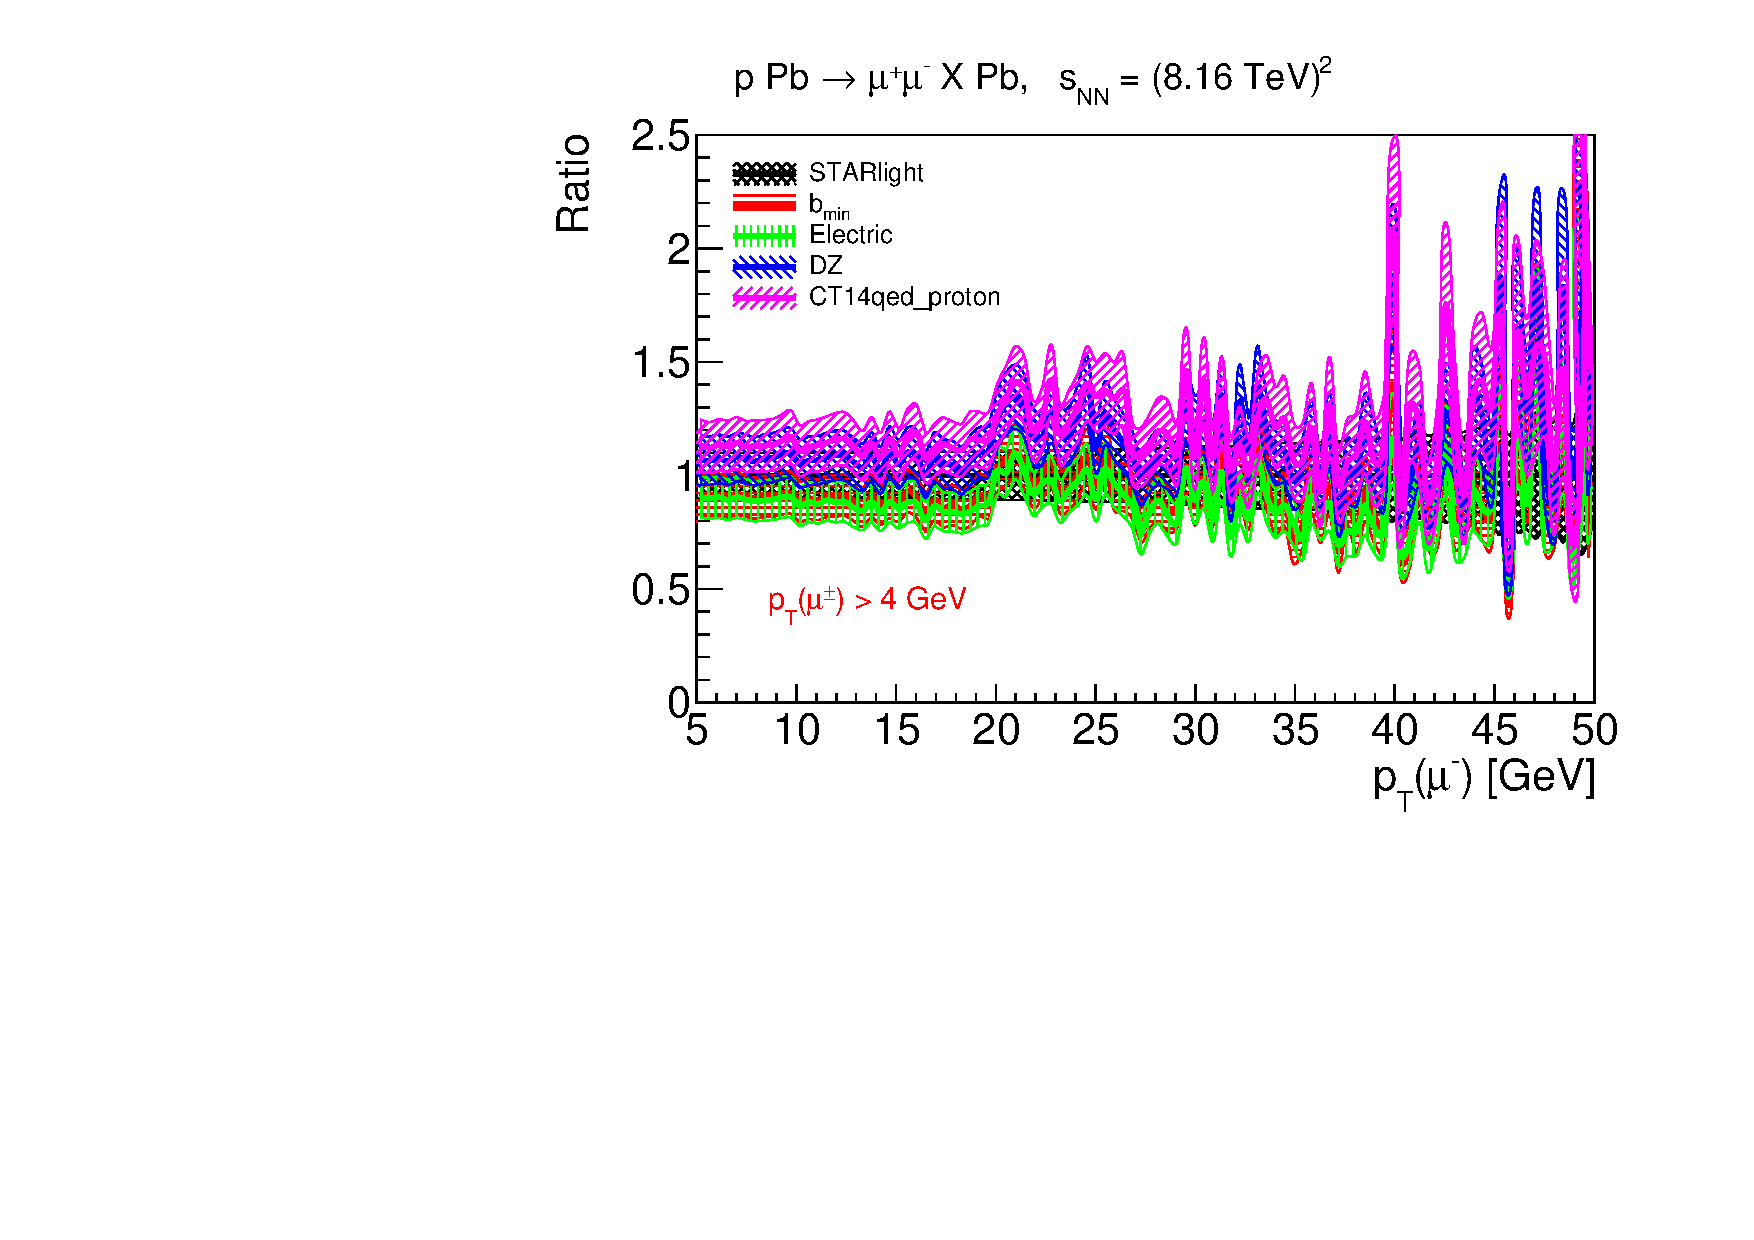
\includegraphics[width=0.4\textwidth]{figures/RatiopTl_elastic.pdf}
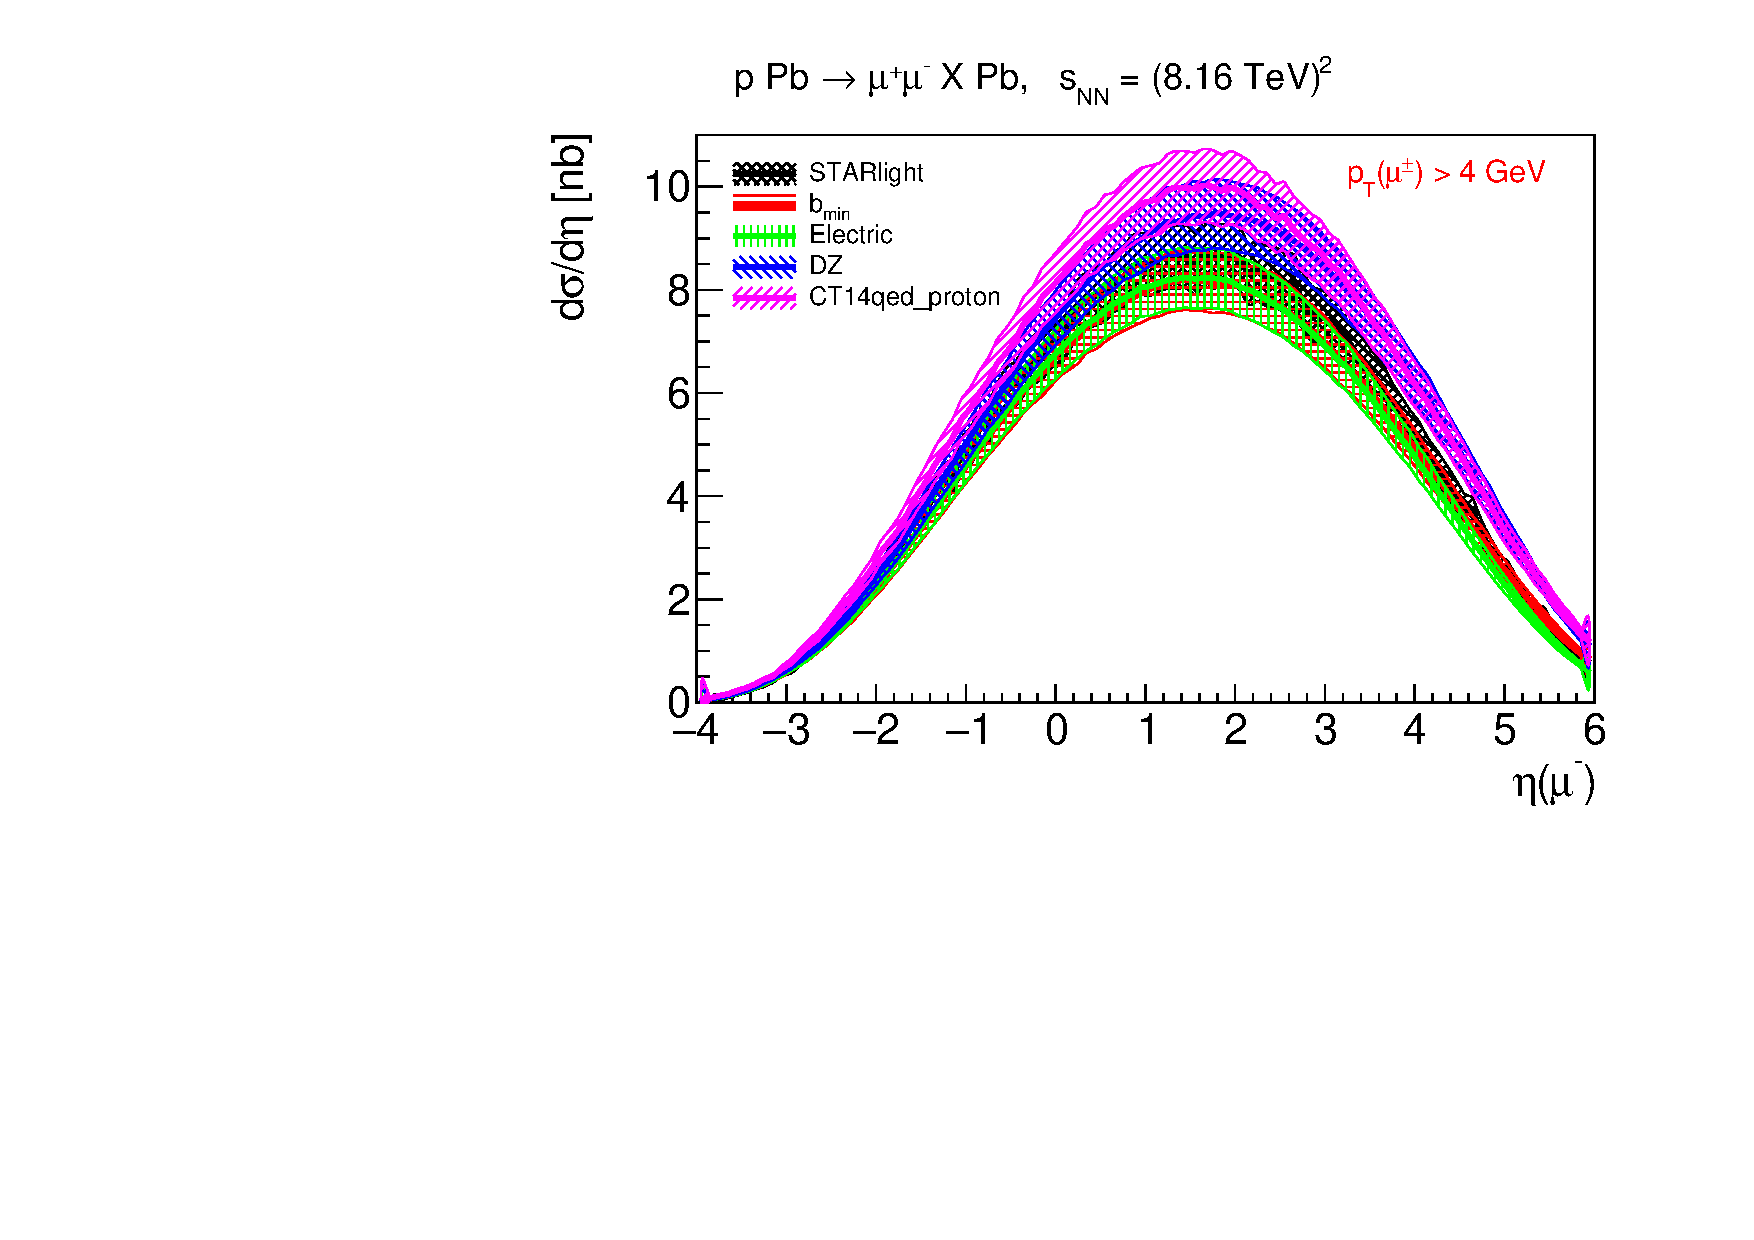
\includegraphics[width=0.4\textwidth]{figures/etal_elastic.pdf}
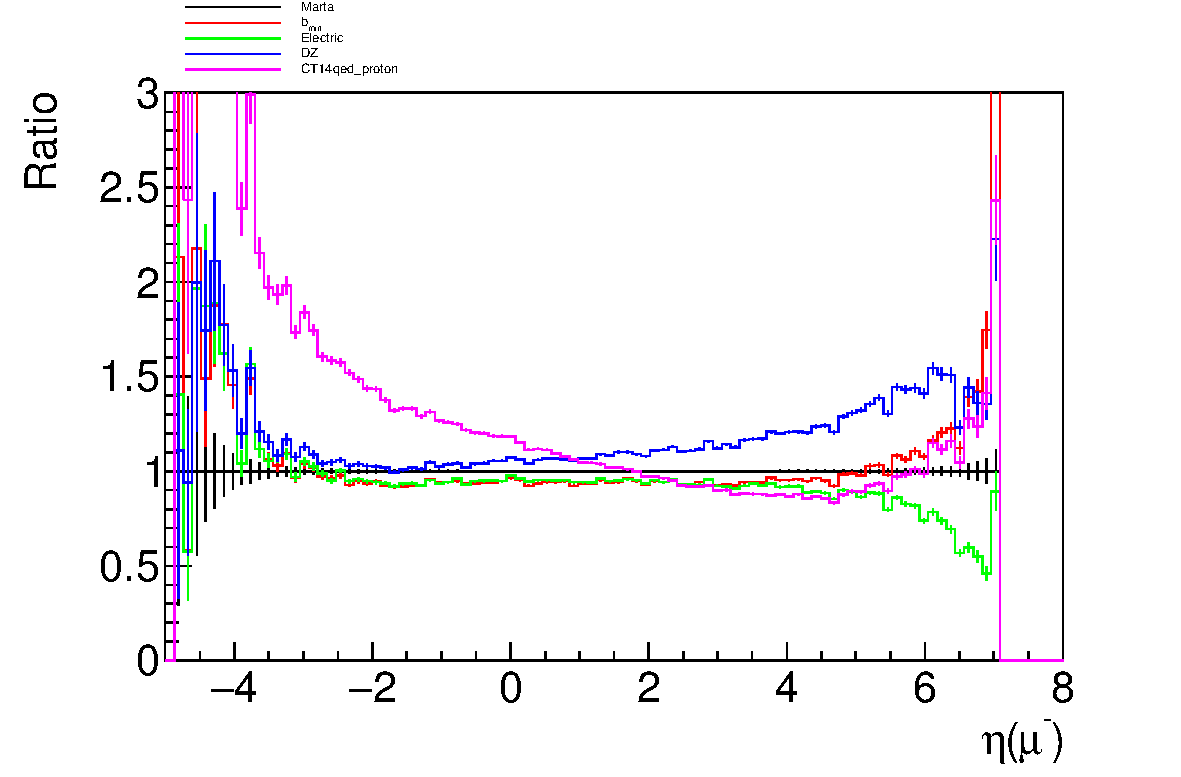
\includegraphics[width=0.4\textwidth]{figures/Ratioetal_elastic.pdf}
\caption{Elastic distributions (the only cut is on leptons $p_T$)}
\label{fig:elastic}
\end{figure}

\begin{figure}[h!]
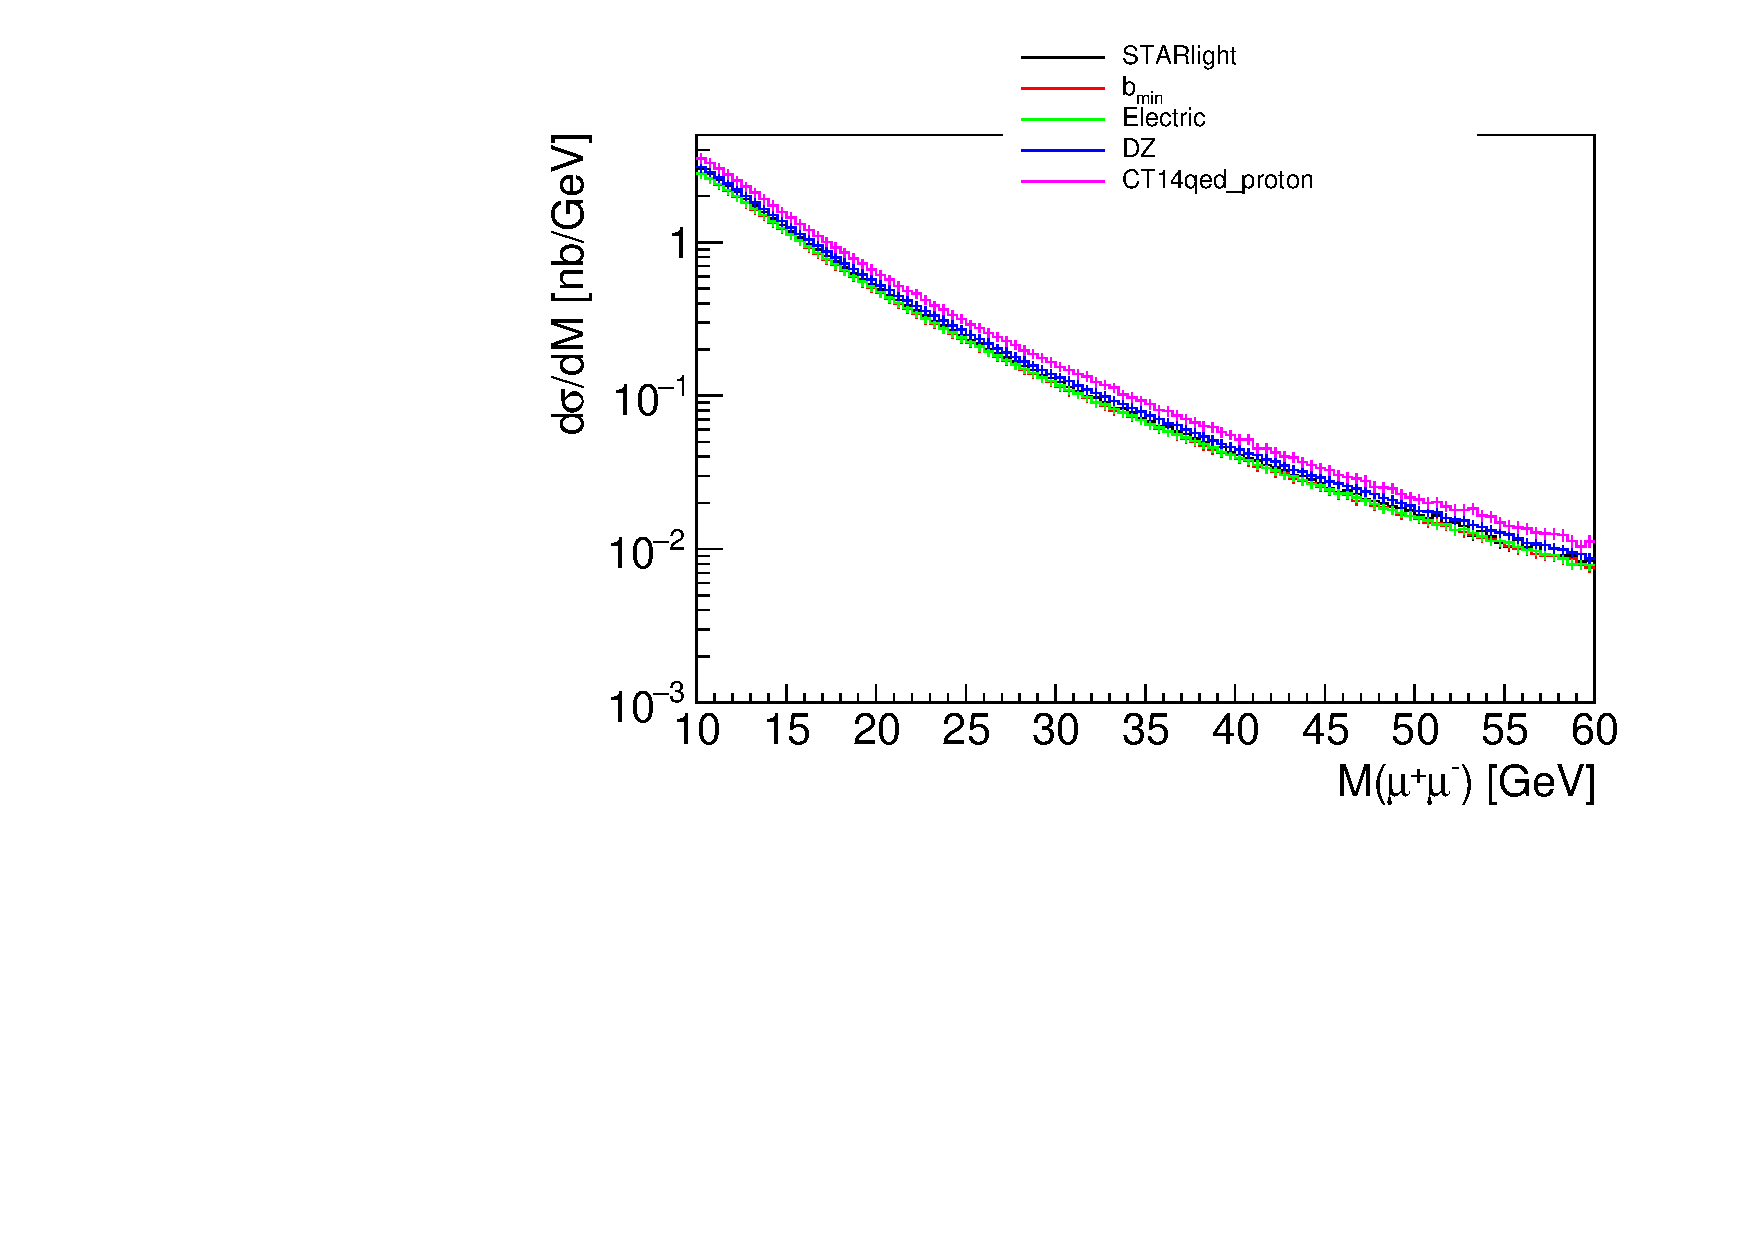
\includegraphics[width=0.4\textwidth]{figures/Mll_elastic_cut.pdf}
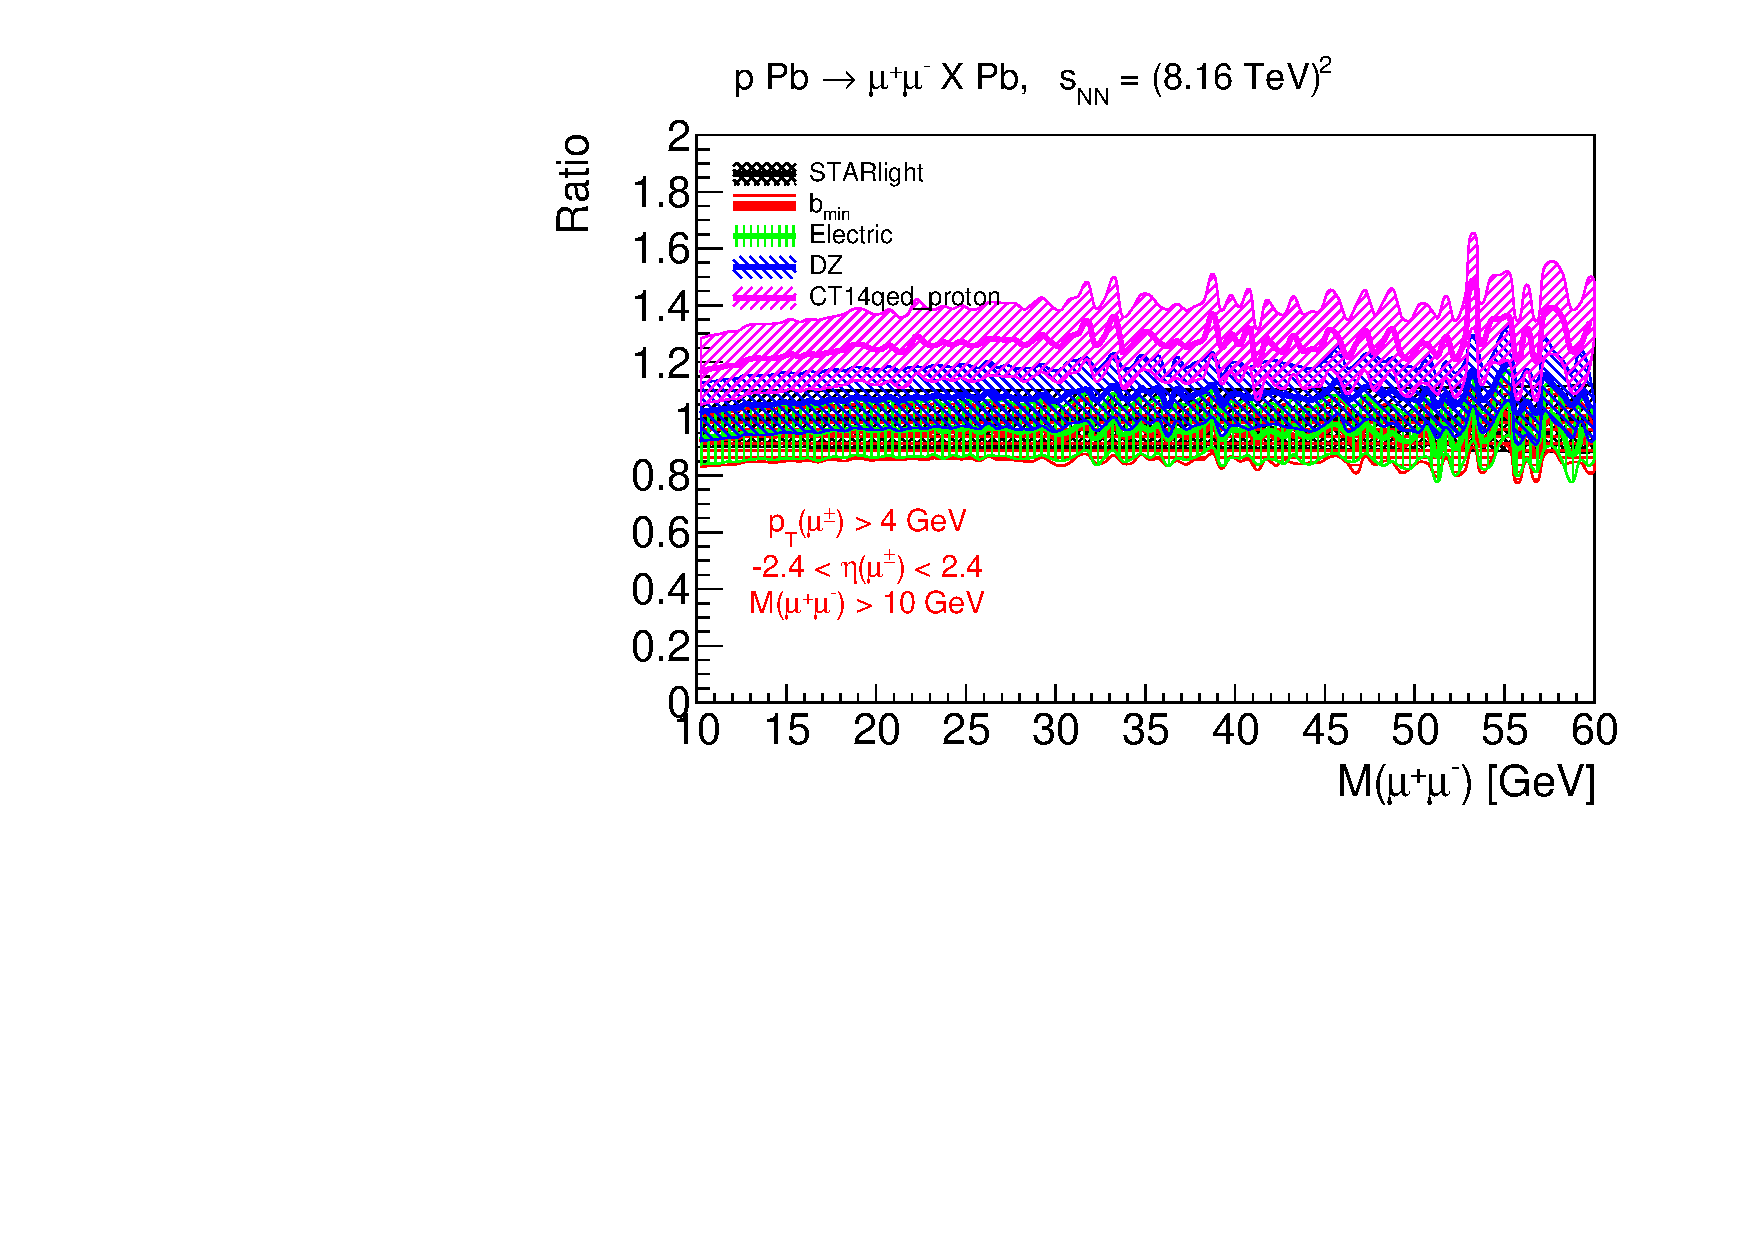
\includegraphics[width=0.4\textwidth]{figures/RatioMll_elastic_cut.pdf}
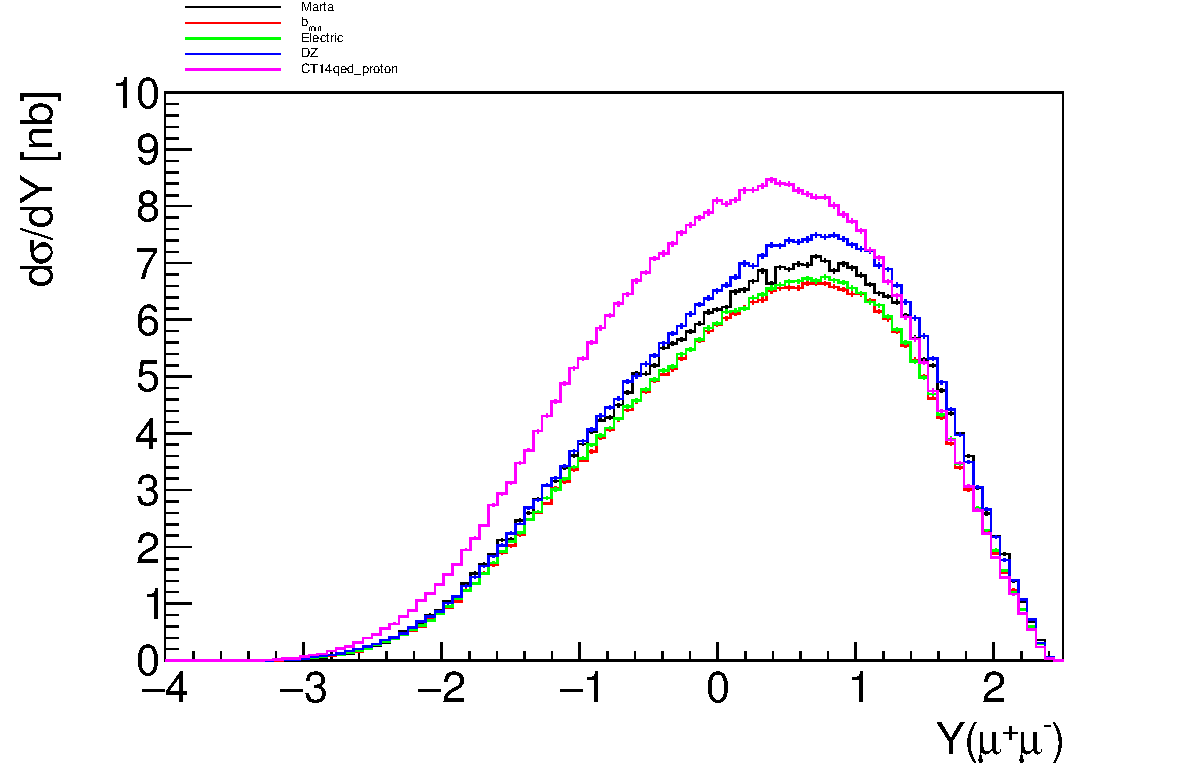
\includegraphics[width=0.4\textwidth]{figures/Yll_elastic_cut.pdf}
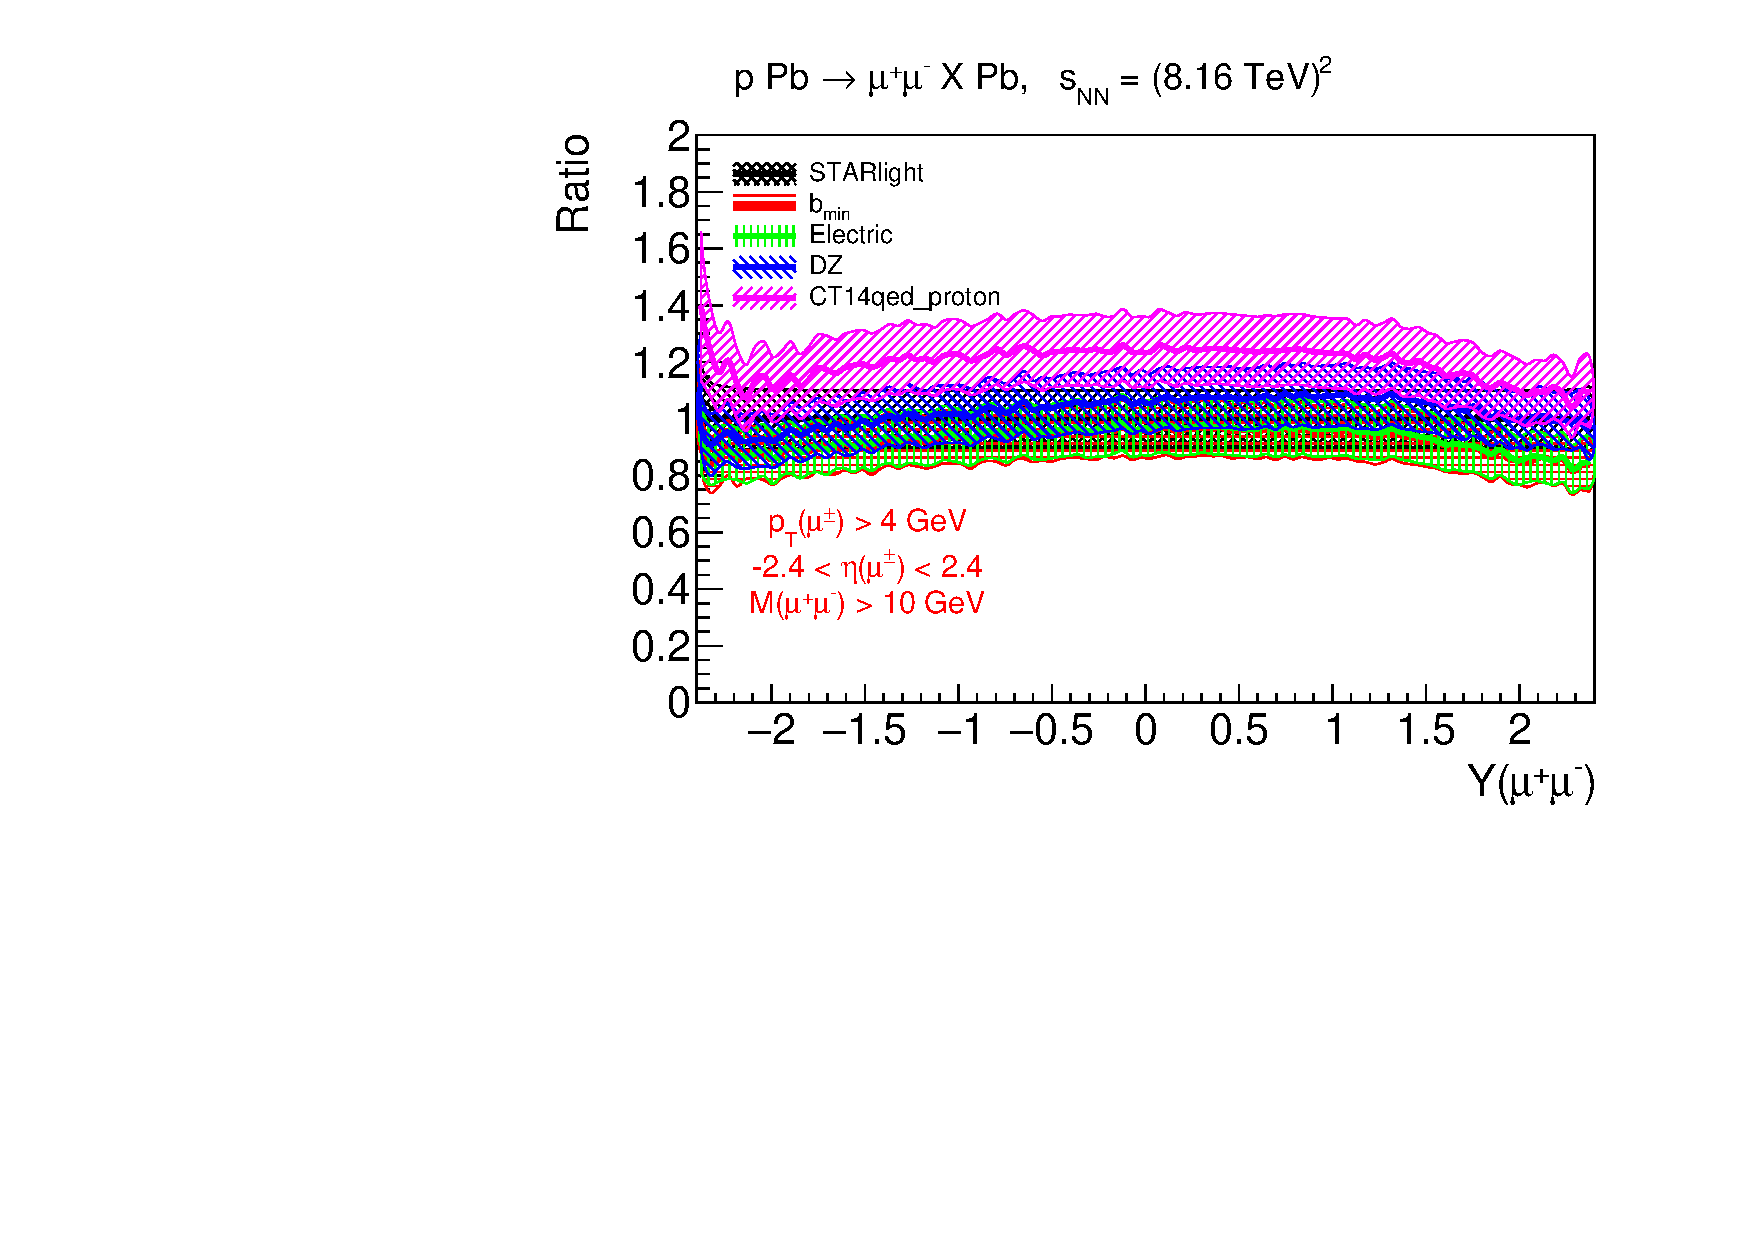
\includegraphics[width=0.4\textwidth]{figures/RatioYll_elastic_cut.pdf}
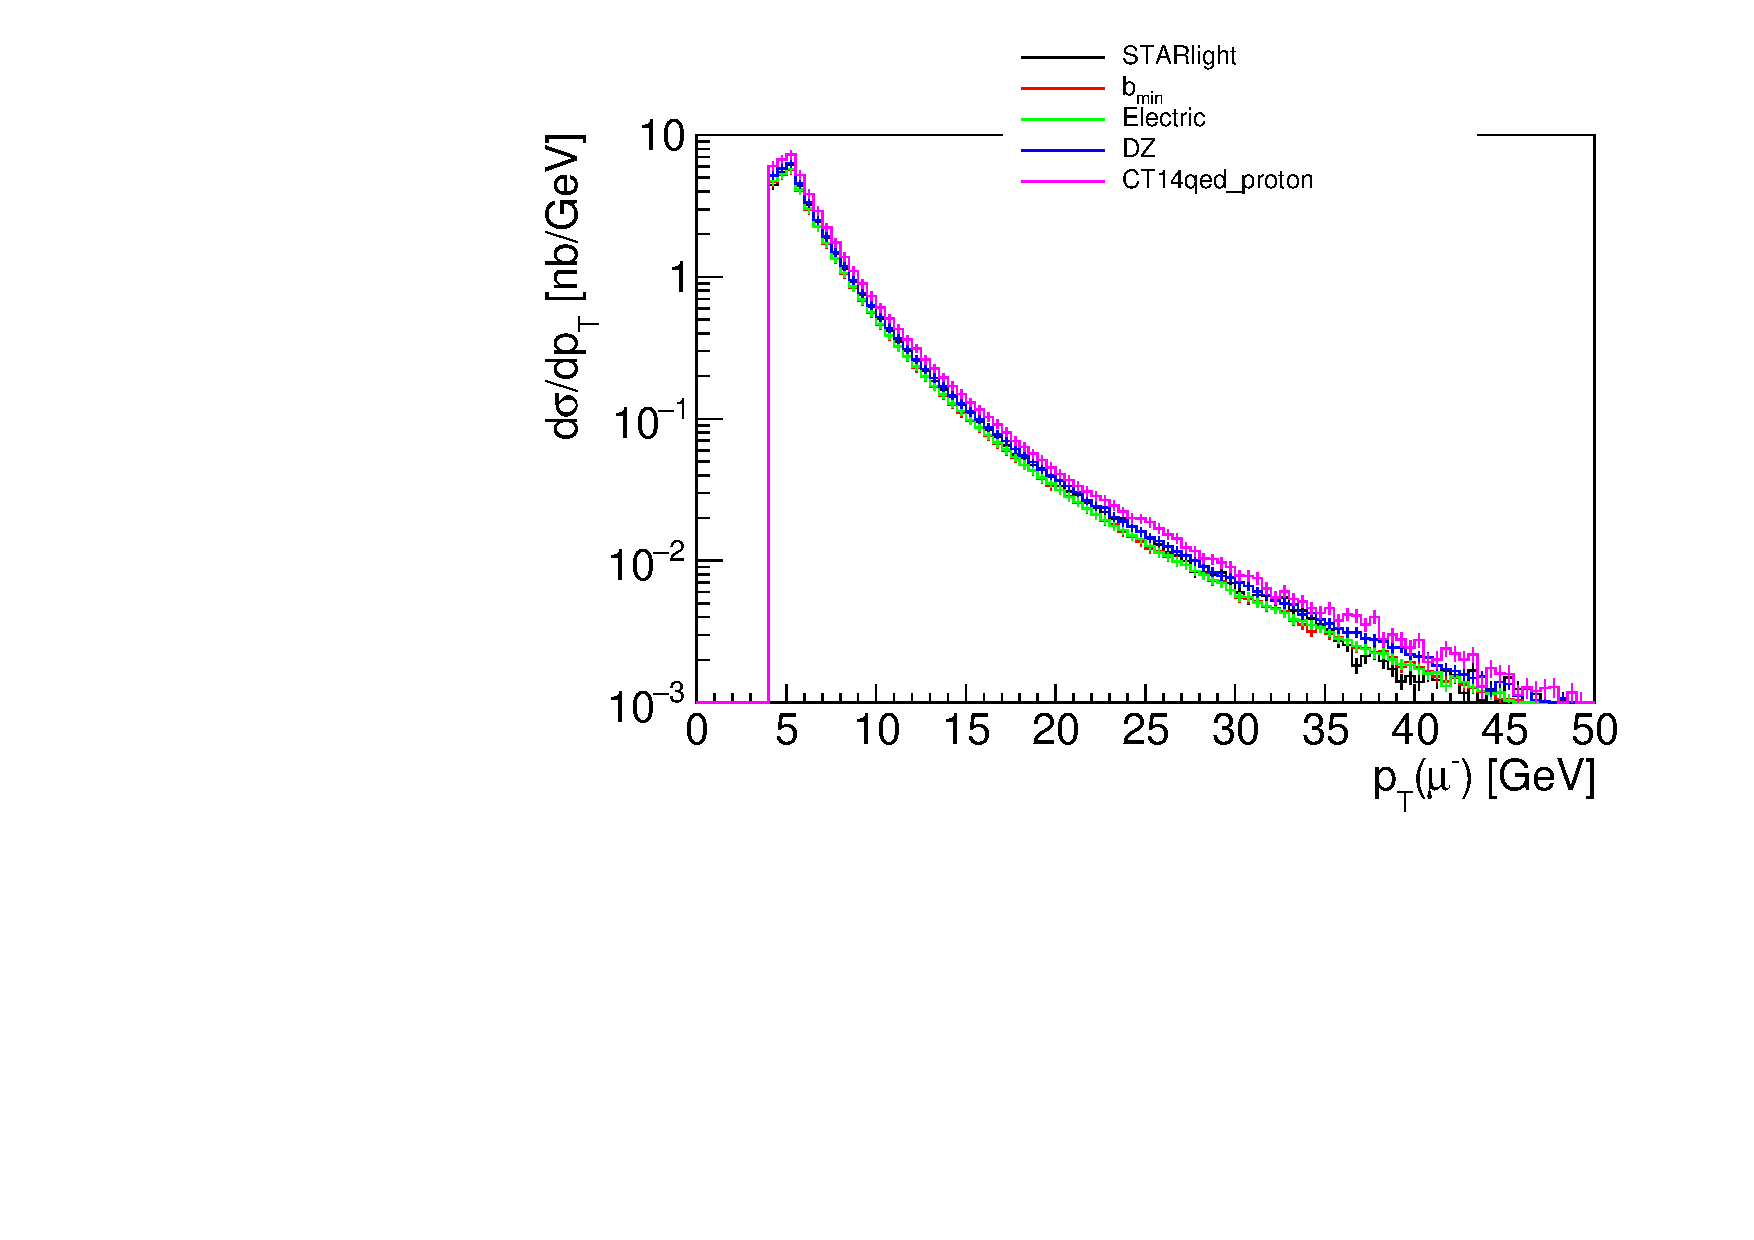
\includegraphics[width=0.4\textwidth]{figures/pTl_elastic_cut.pdf}
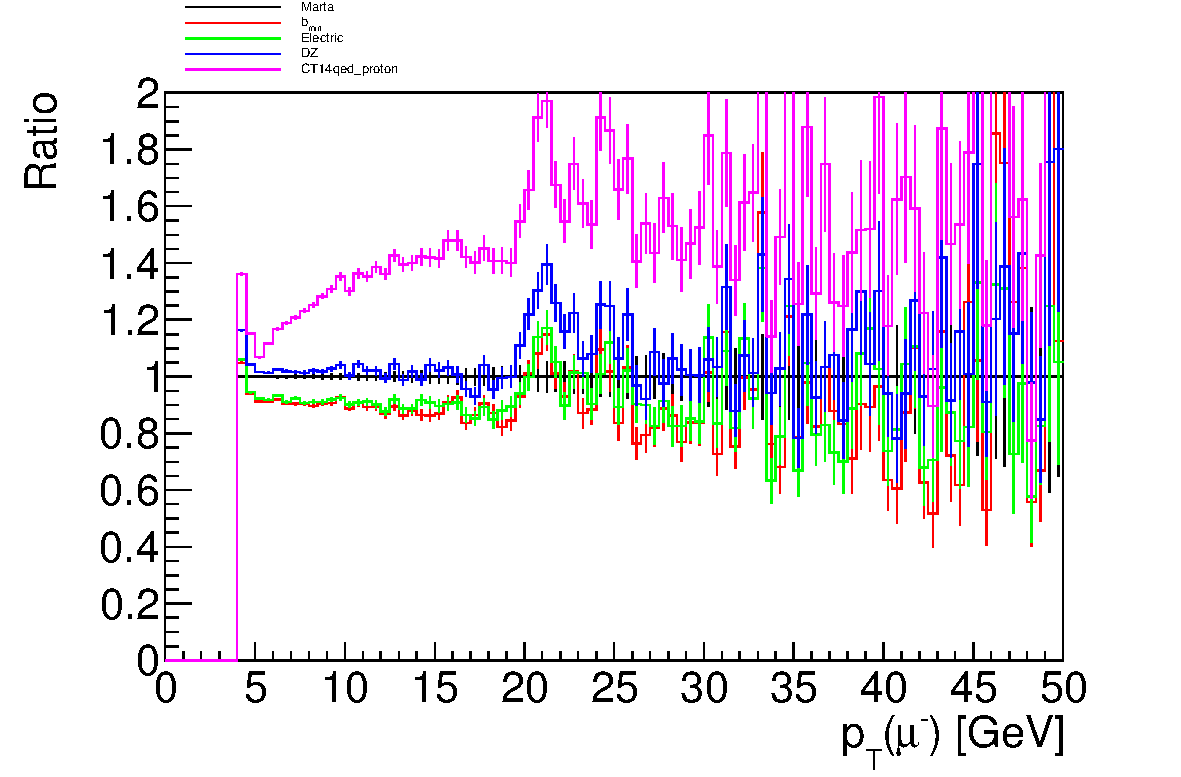
\includegraphics[width=0.4\textwidth]{figures/RatiopTl_elastic_cut.pdf}
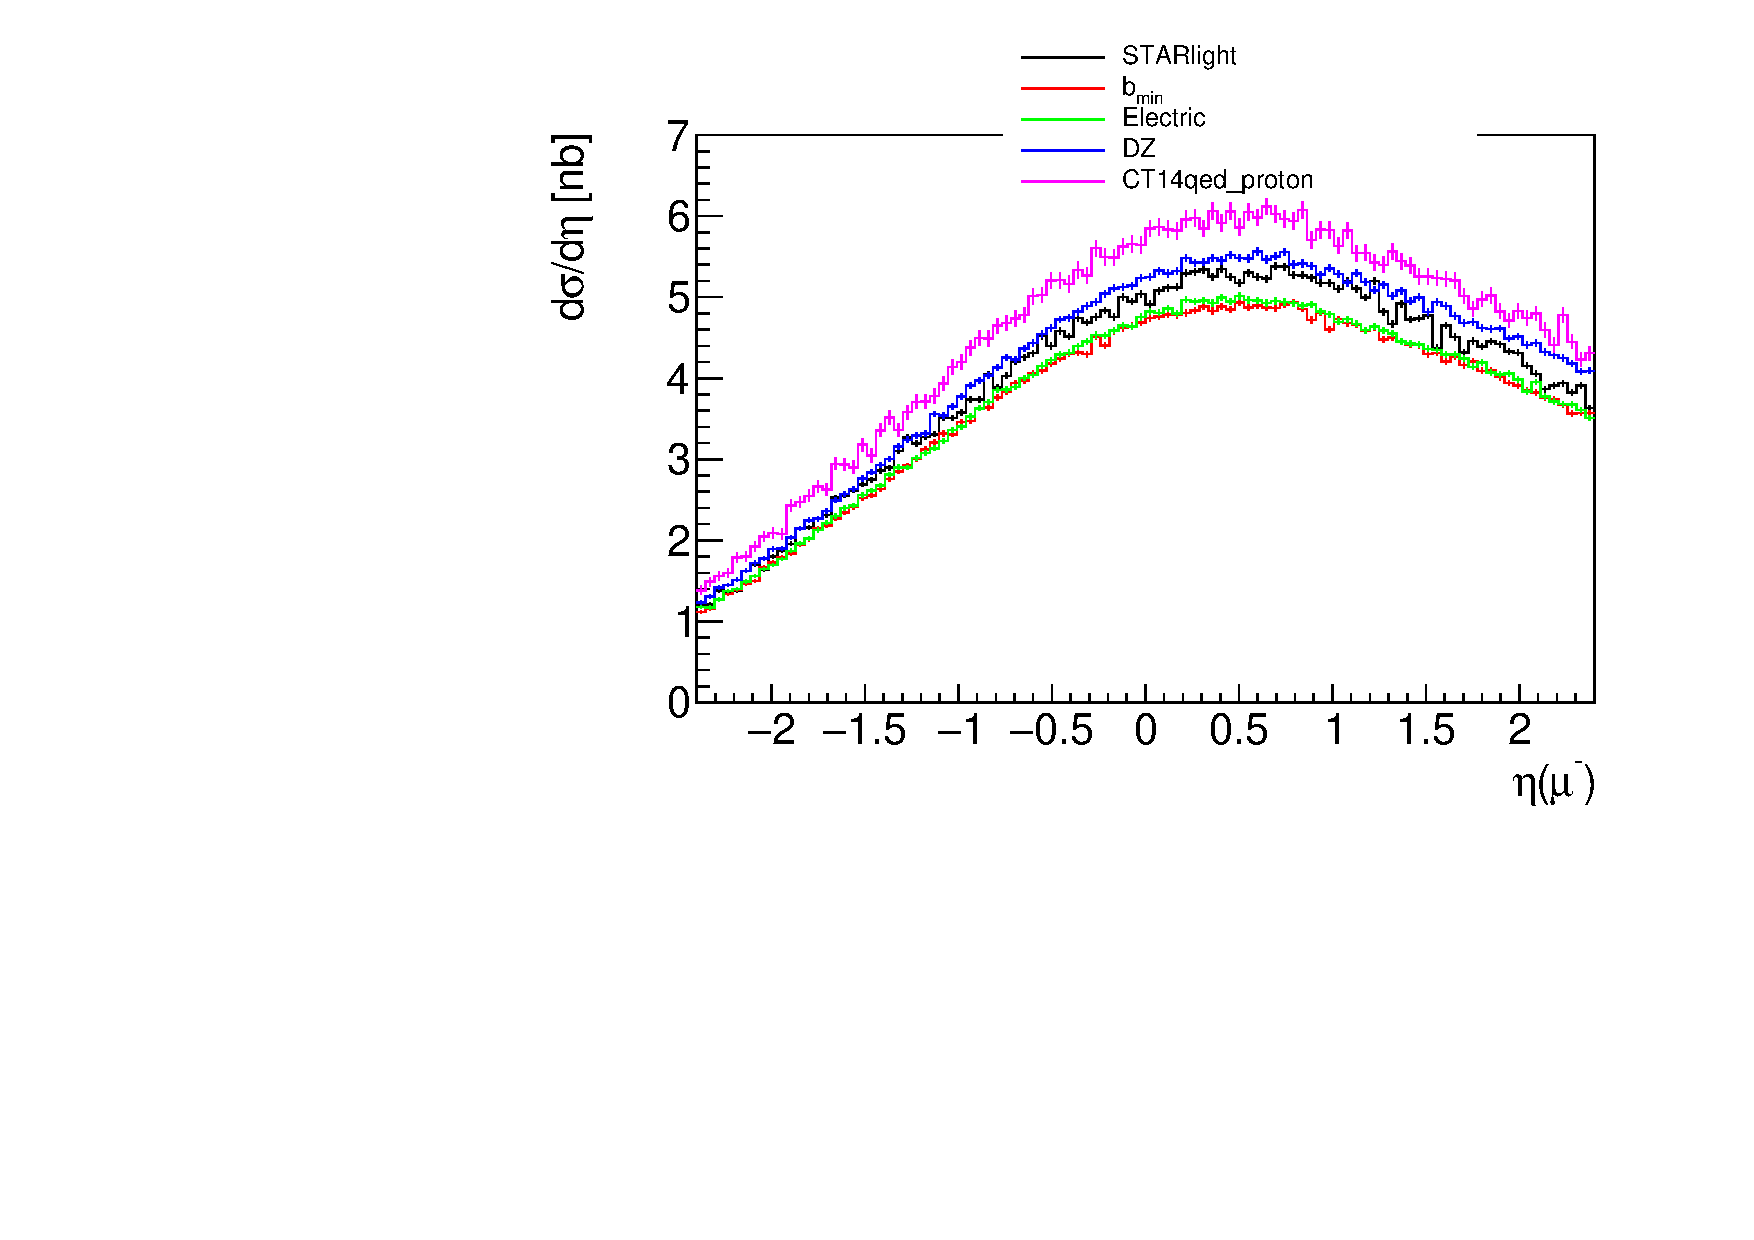
\includegraphics[width=0.4\textwidth]{figures/etal_elastic_cut.pdf}
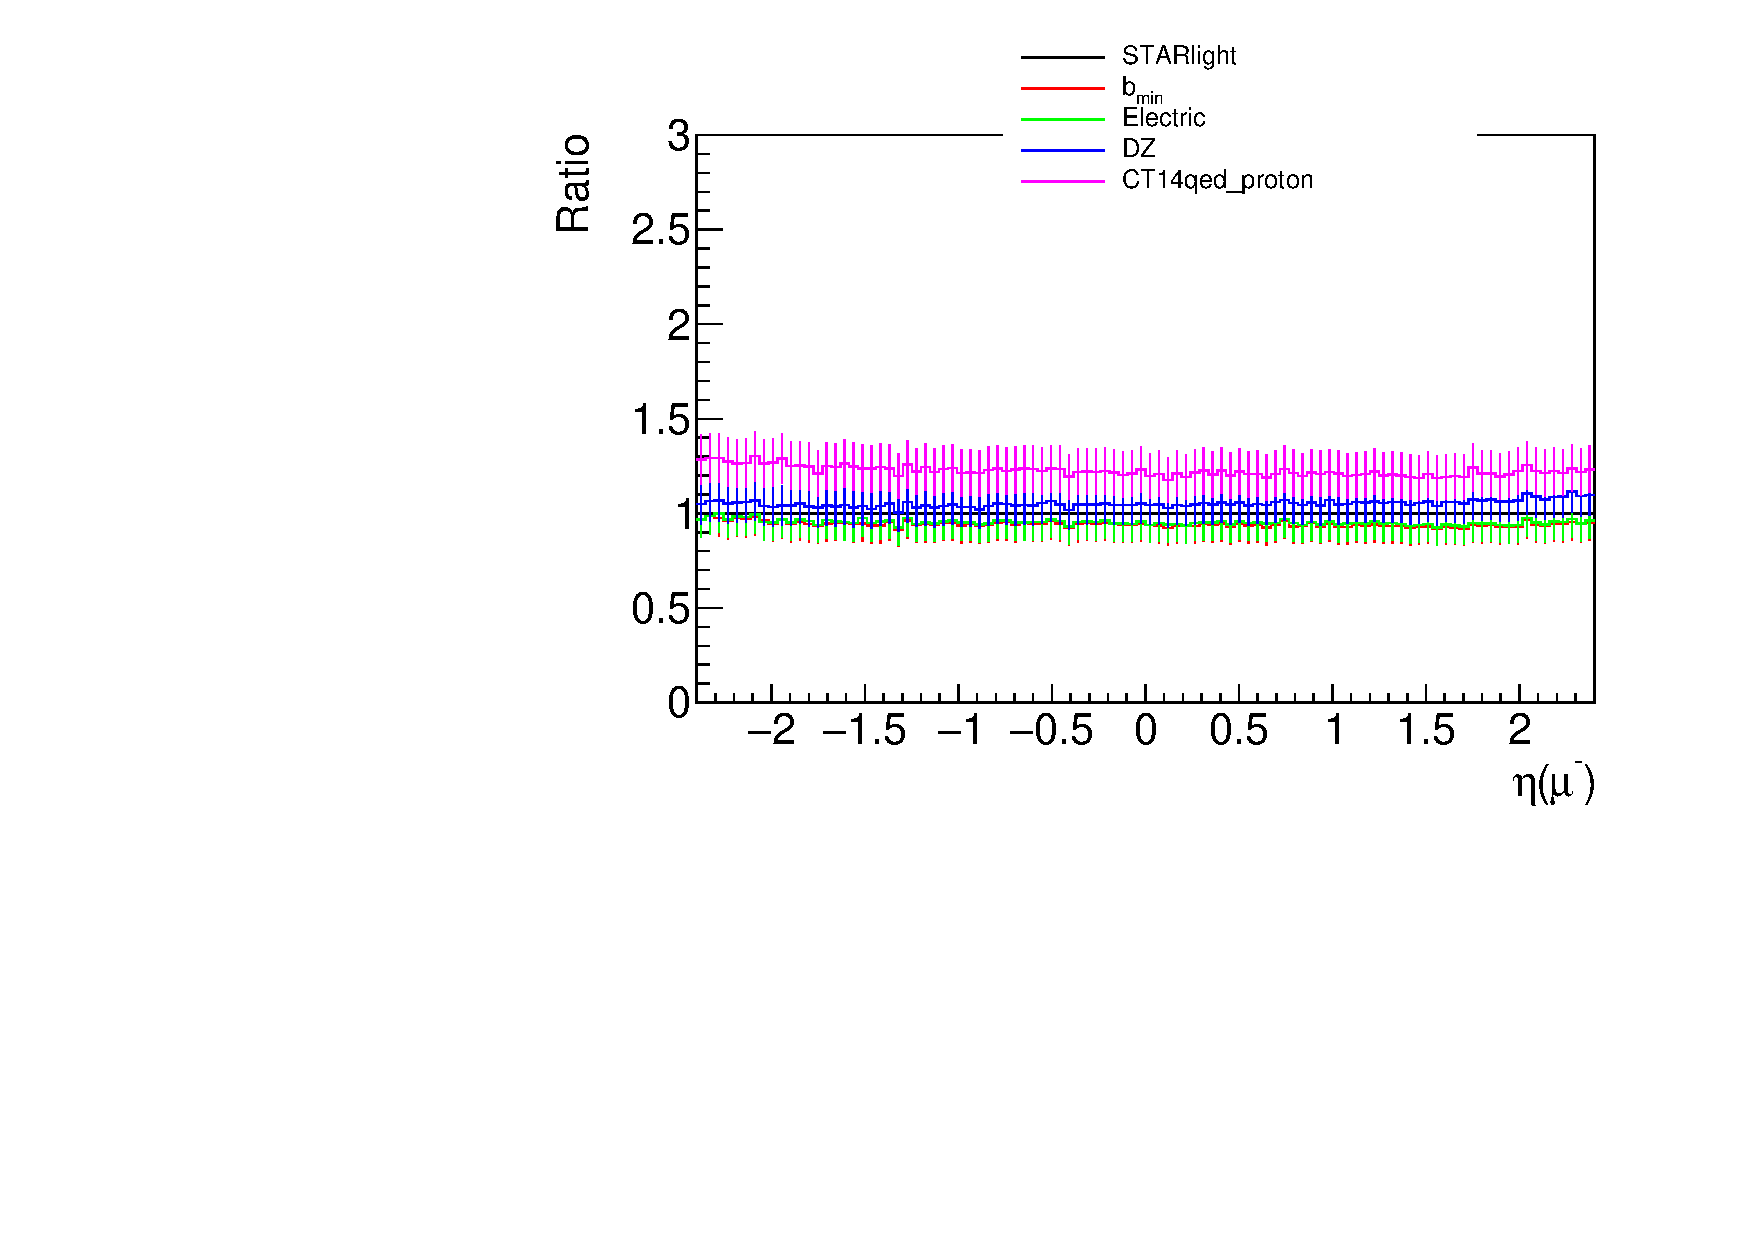
\includegraphics[width=0.4\textwidth]{figures/Ratioetal_elastic_cut.pdf}
\caption{Elastic distributions (fiducial region)}
\label{fig:elastic_cut}
\end{figure}

\begin{figure}[h!]
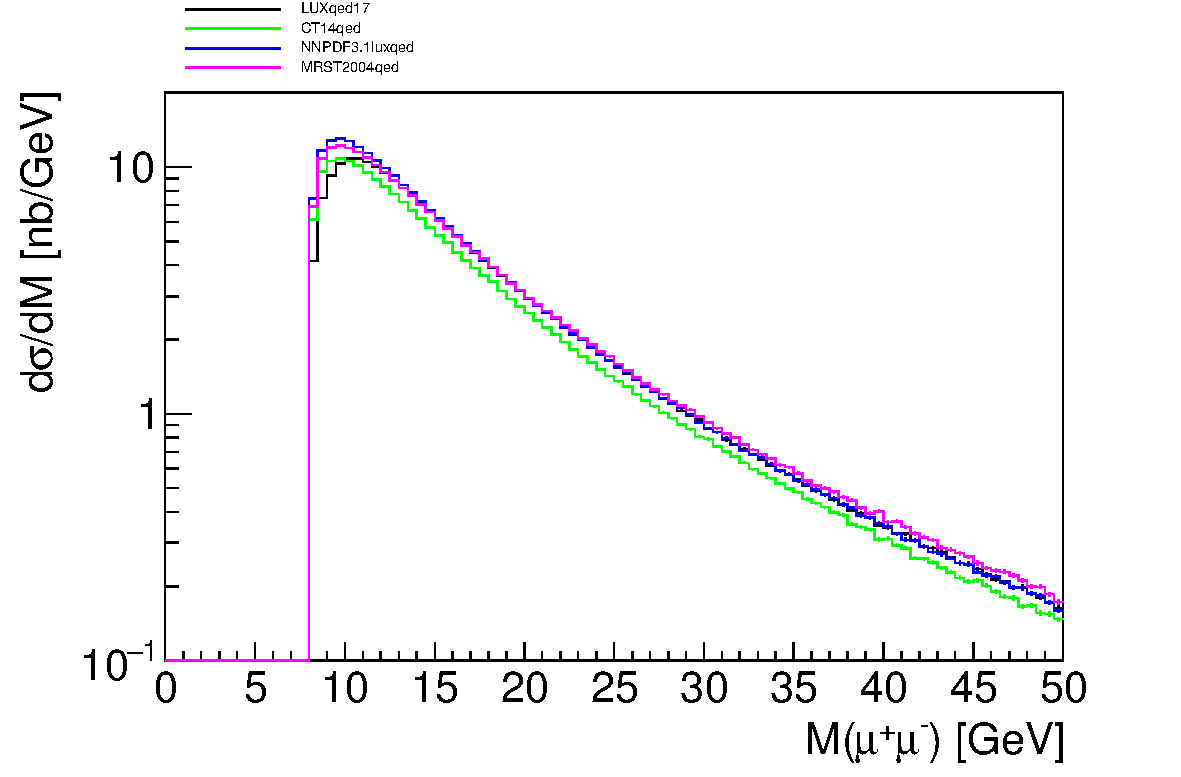
\includegraphics[width=0.4\textwidth]{figures/Mll_inc.pdf}
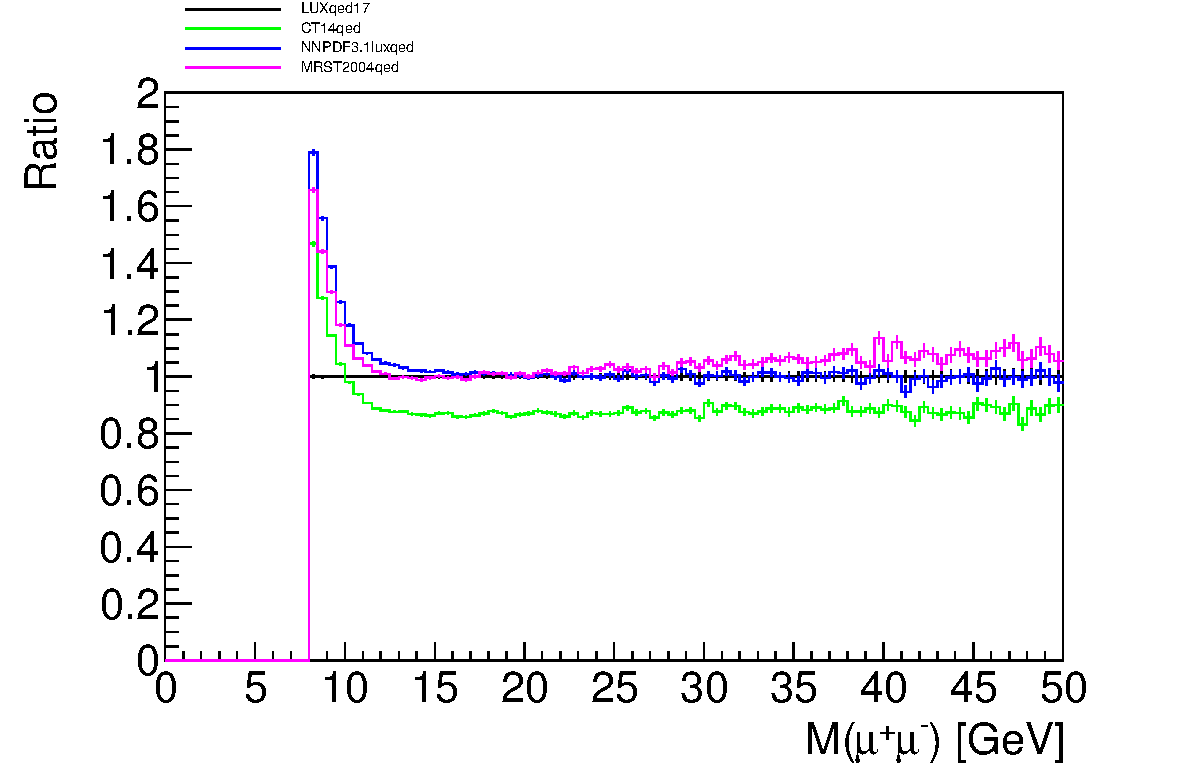
\includegraphics[width=0.4\textwidth]{figures/RatioMll_inc.pdf}
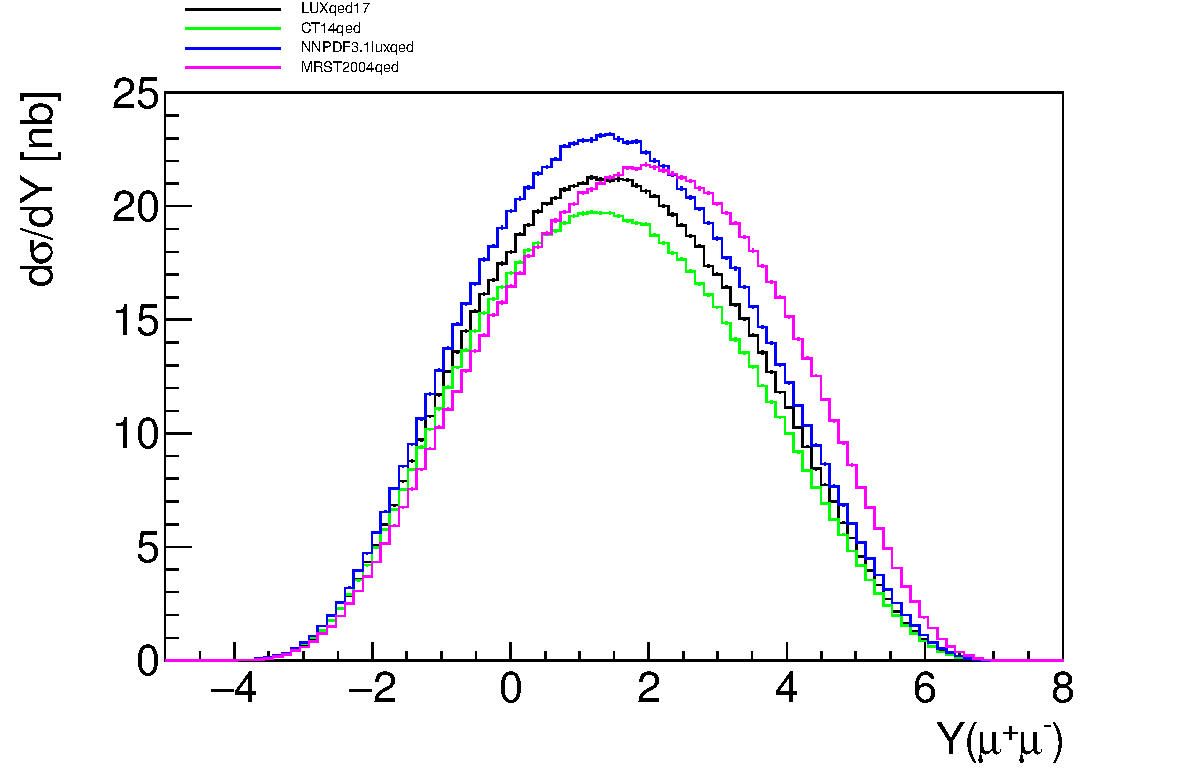
\includegraphics[width=0.4\textwidth]{figures/Yll_inc.pdf}
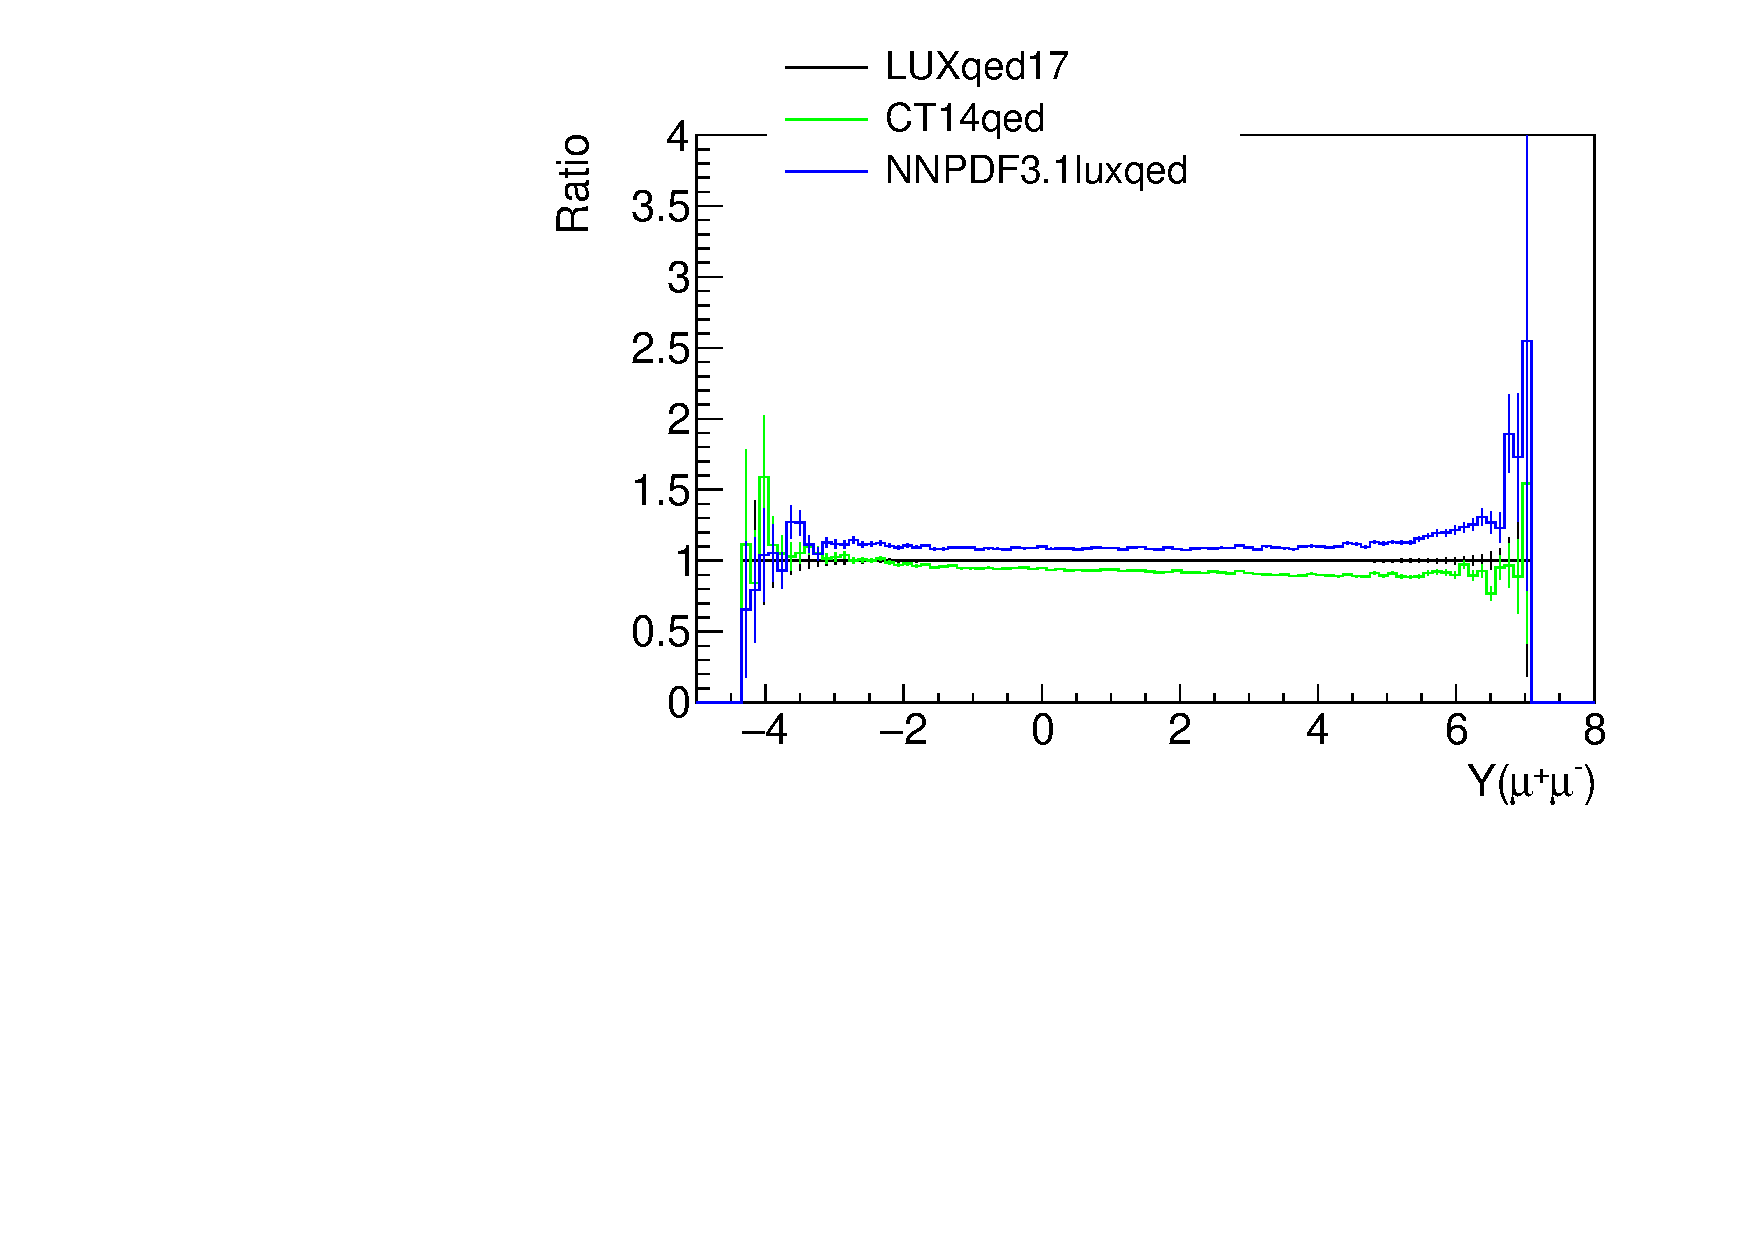
\includegraphics[width=0.4\textwidth]{figures/RatioYll_inc.pdf}
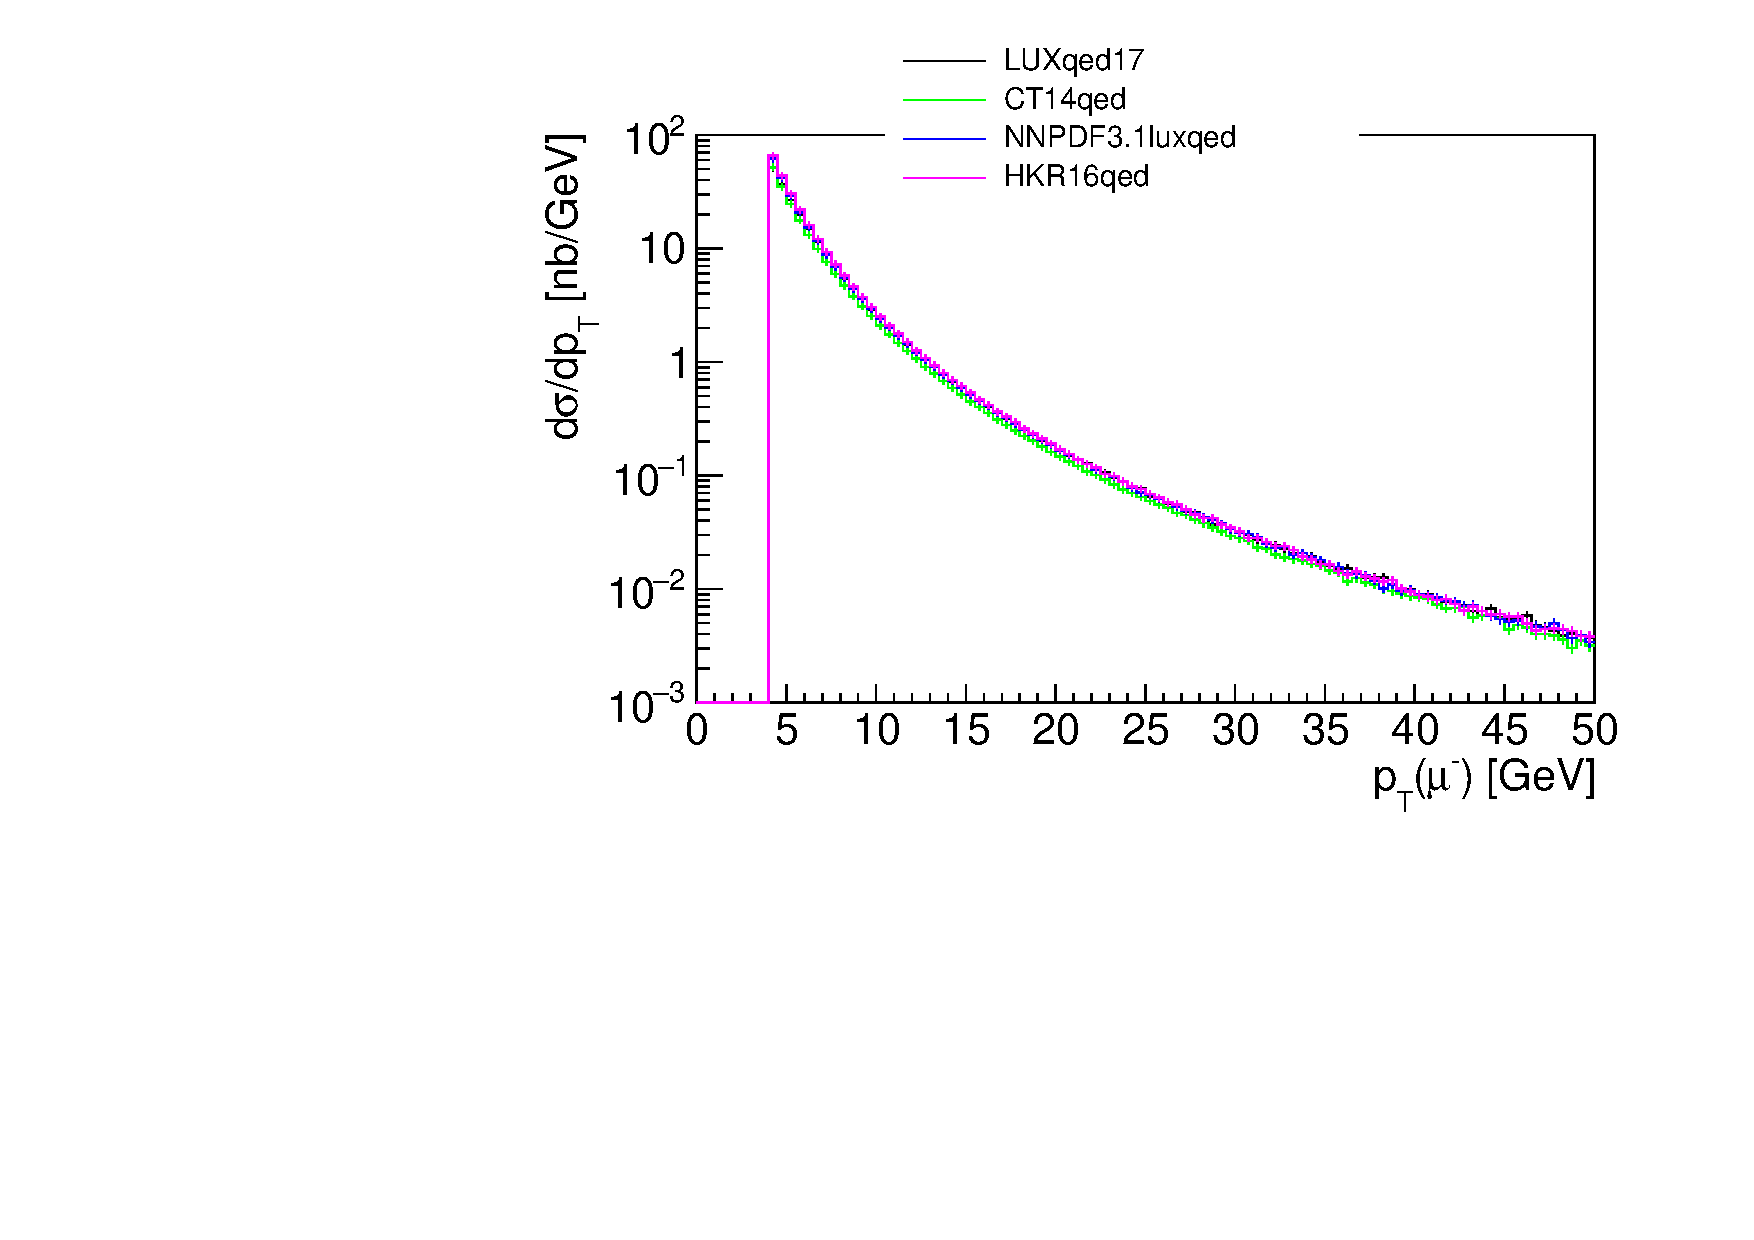
\includegraphics[width=0.4\textwidth]{figures/pTl_inc.pdf}
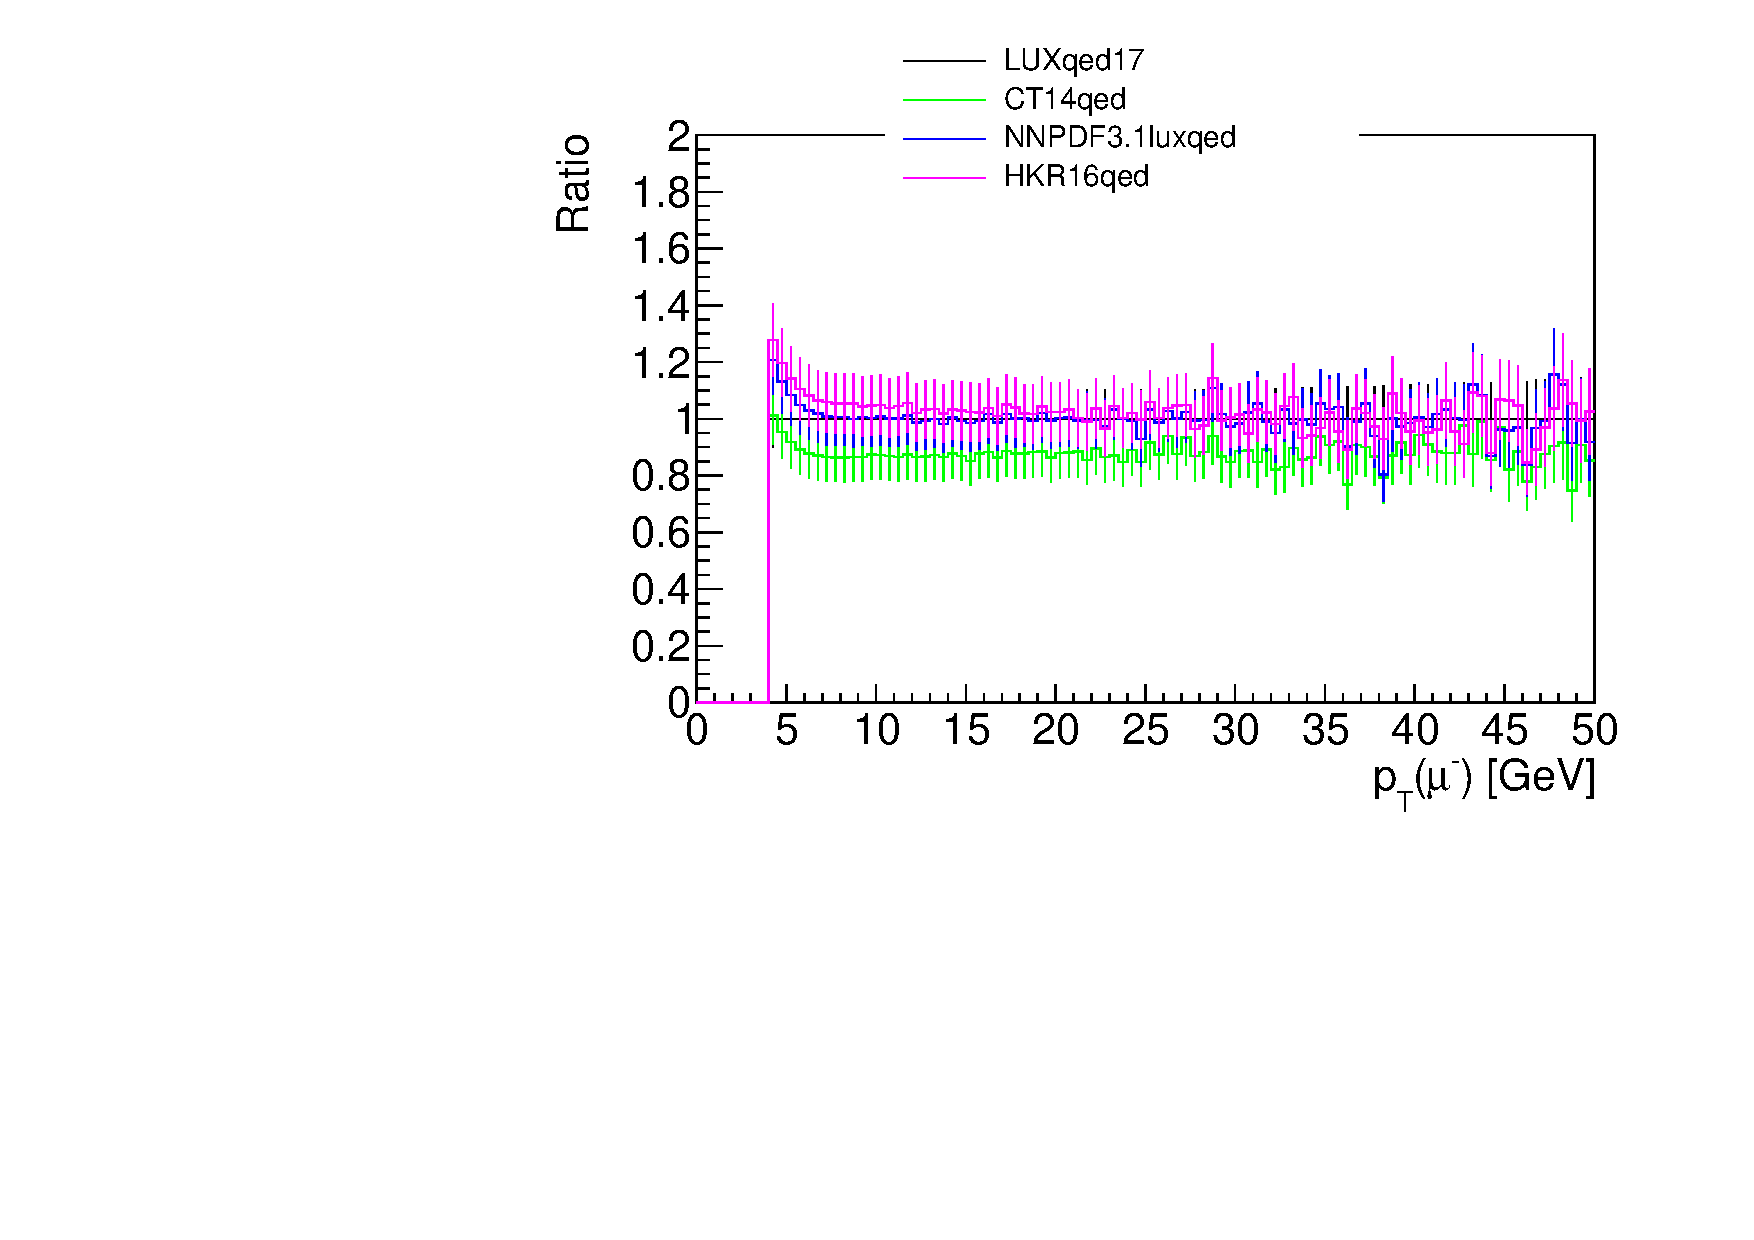
\includegraphics[width=0.4\textwidth]{figures/RatiopTl_inc.pdf}
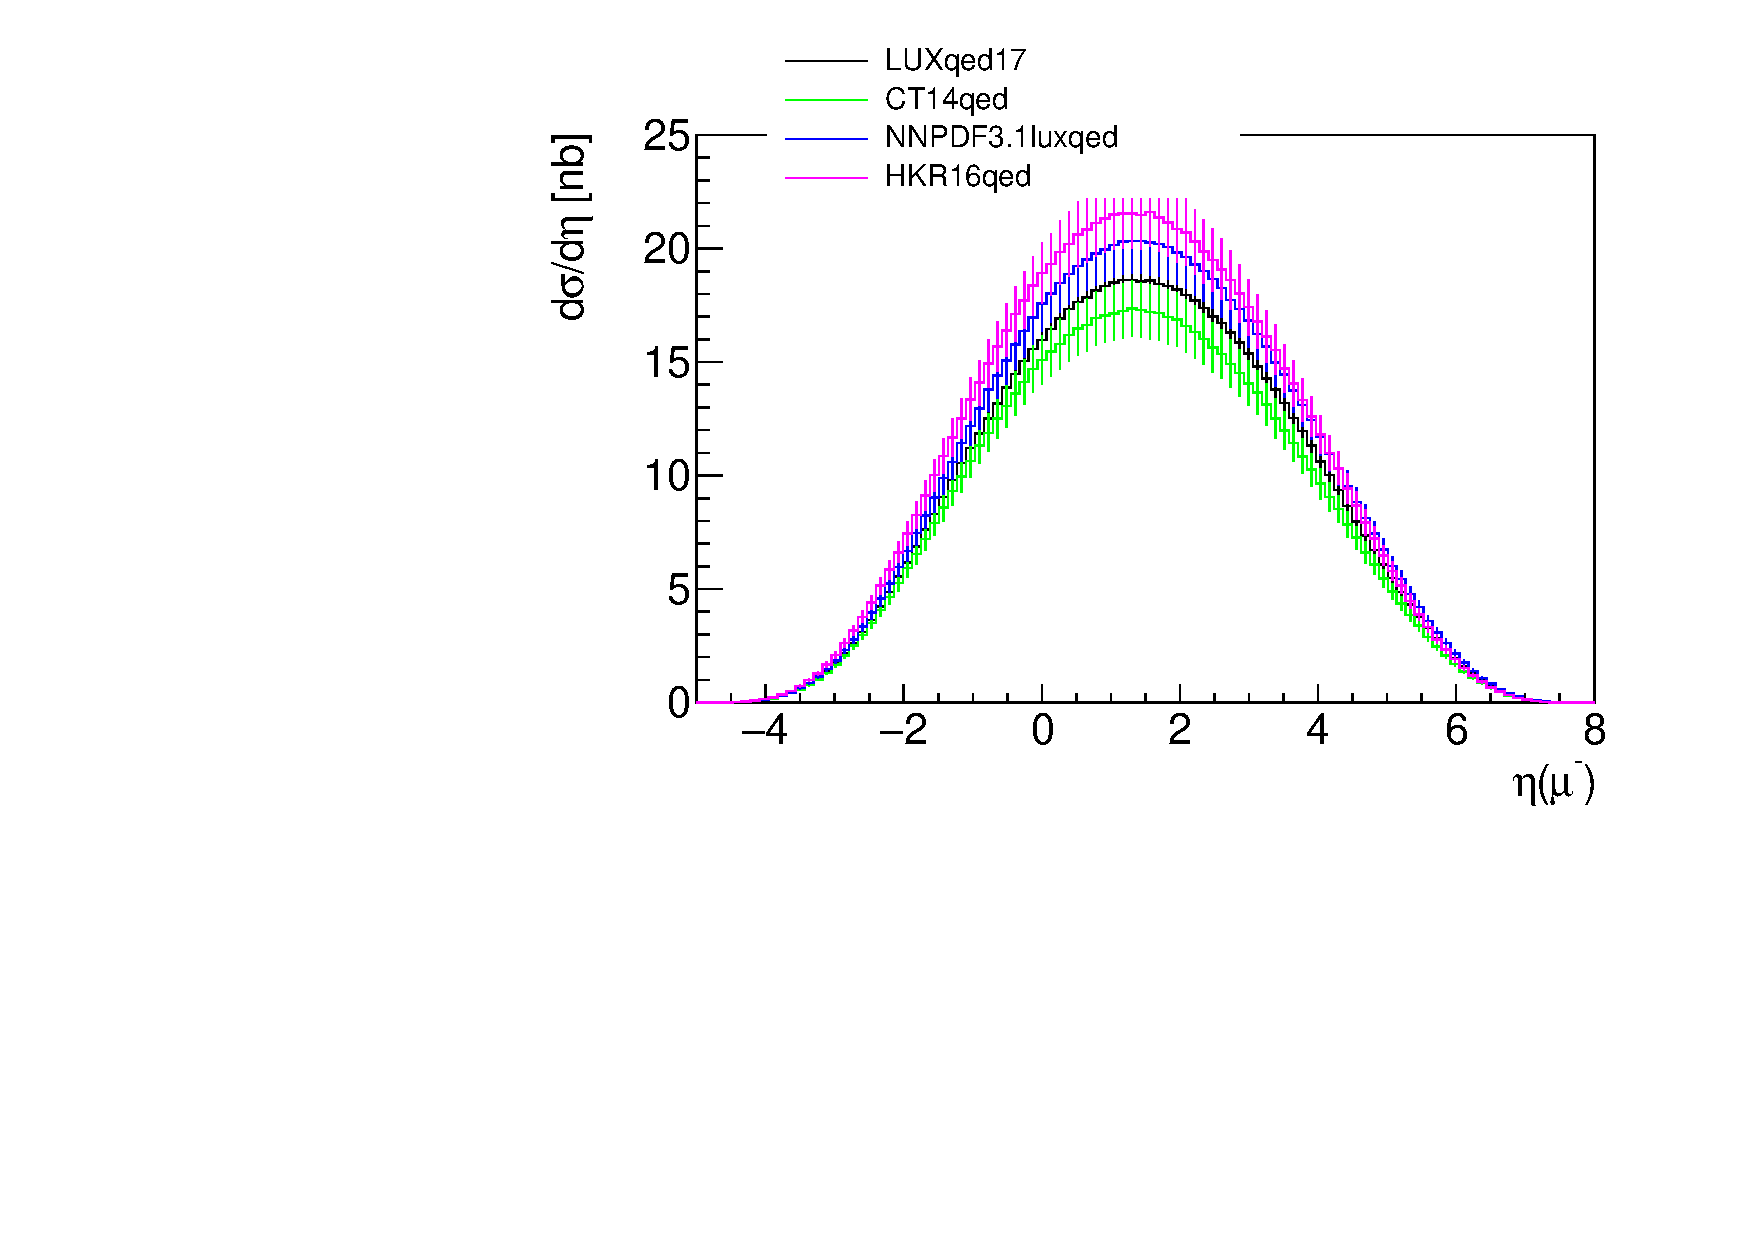
\includegraphics[width=0.4\textwidth]{figures/etal_inc.pdf}
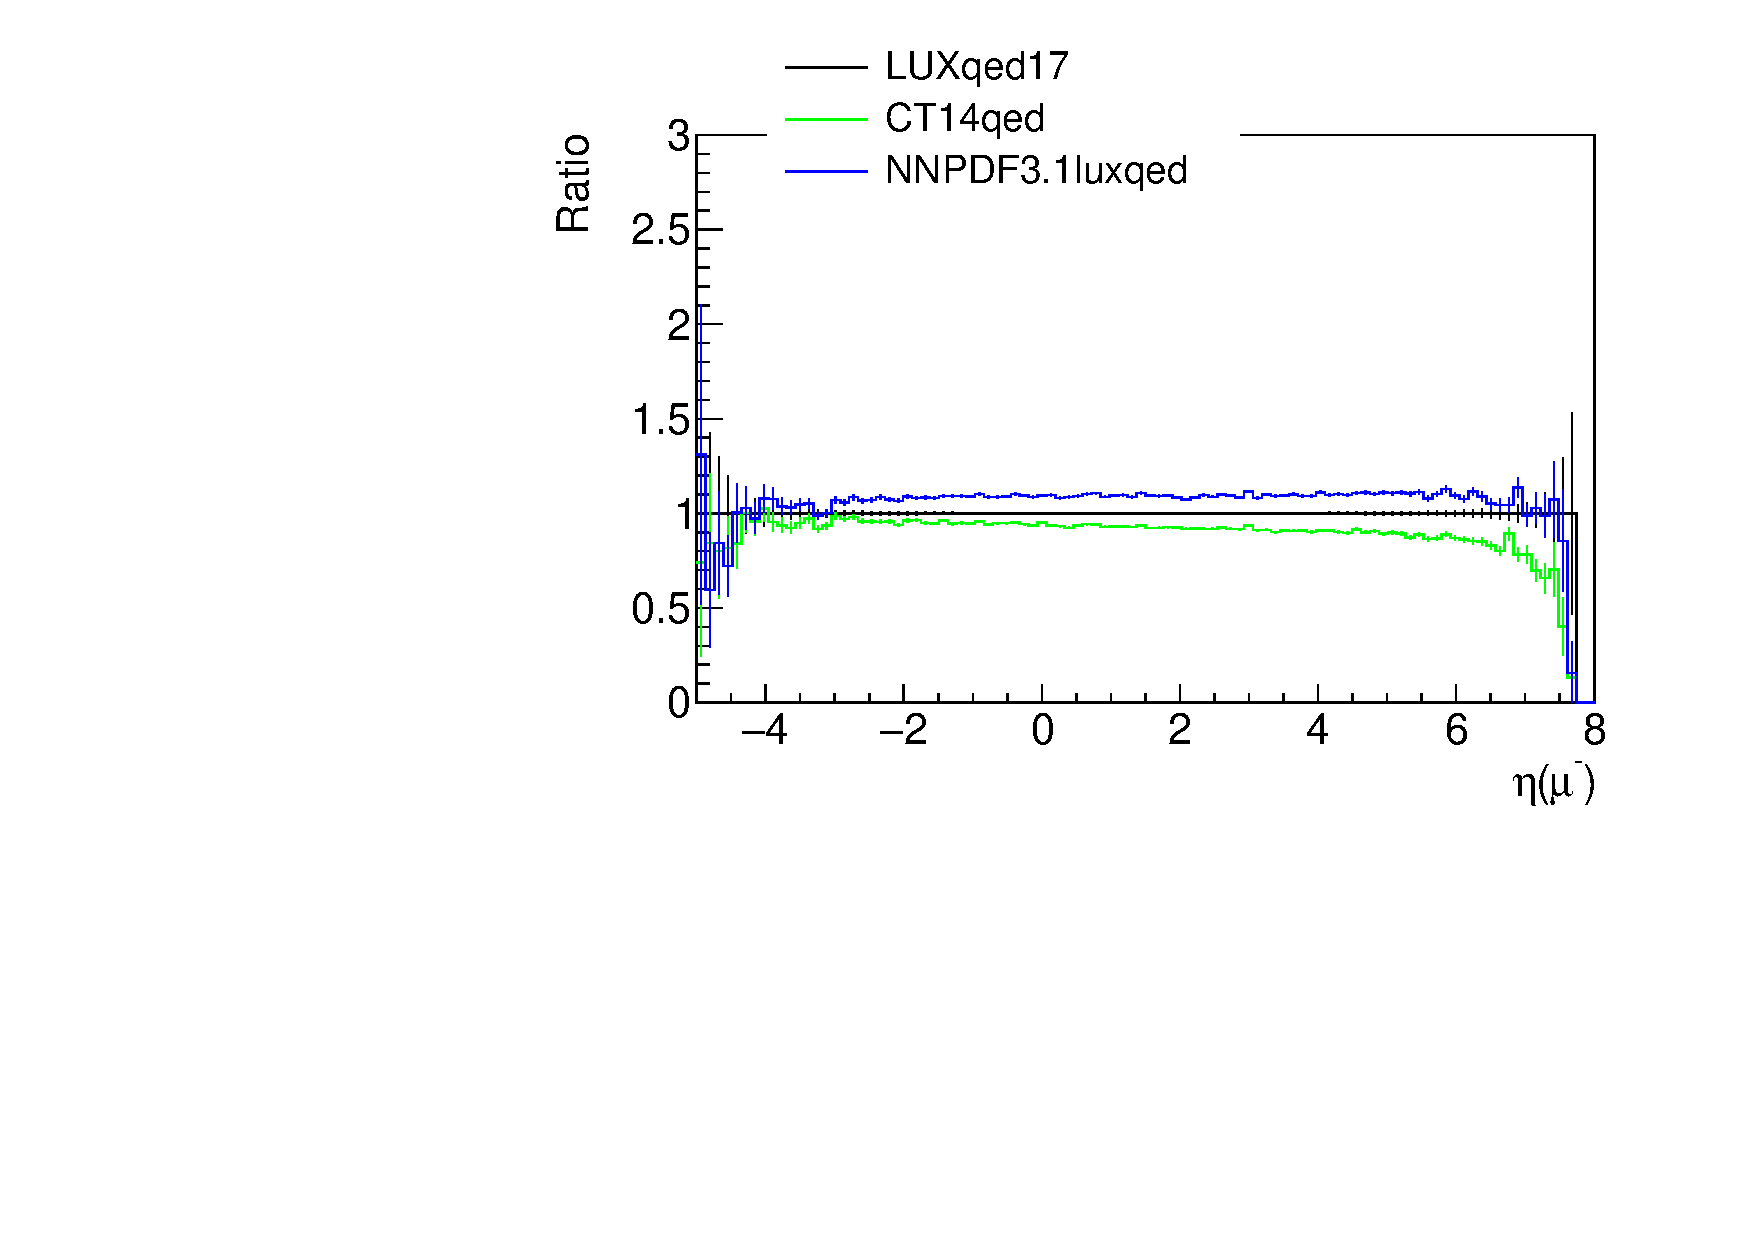
\includegraphics[width=0.4\textwidth]{figures/Ratioetal_inc.pdf}
\caption{Inclusive distributions (the only cut is on leptons $p_T$)}
\label{fig:inc}
\end{figure}

\begin{figure}[h!]
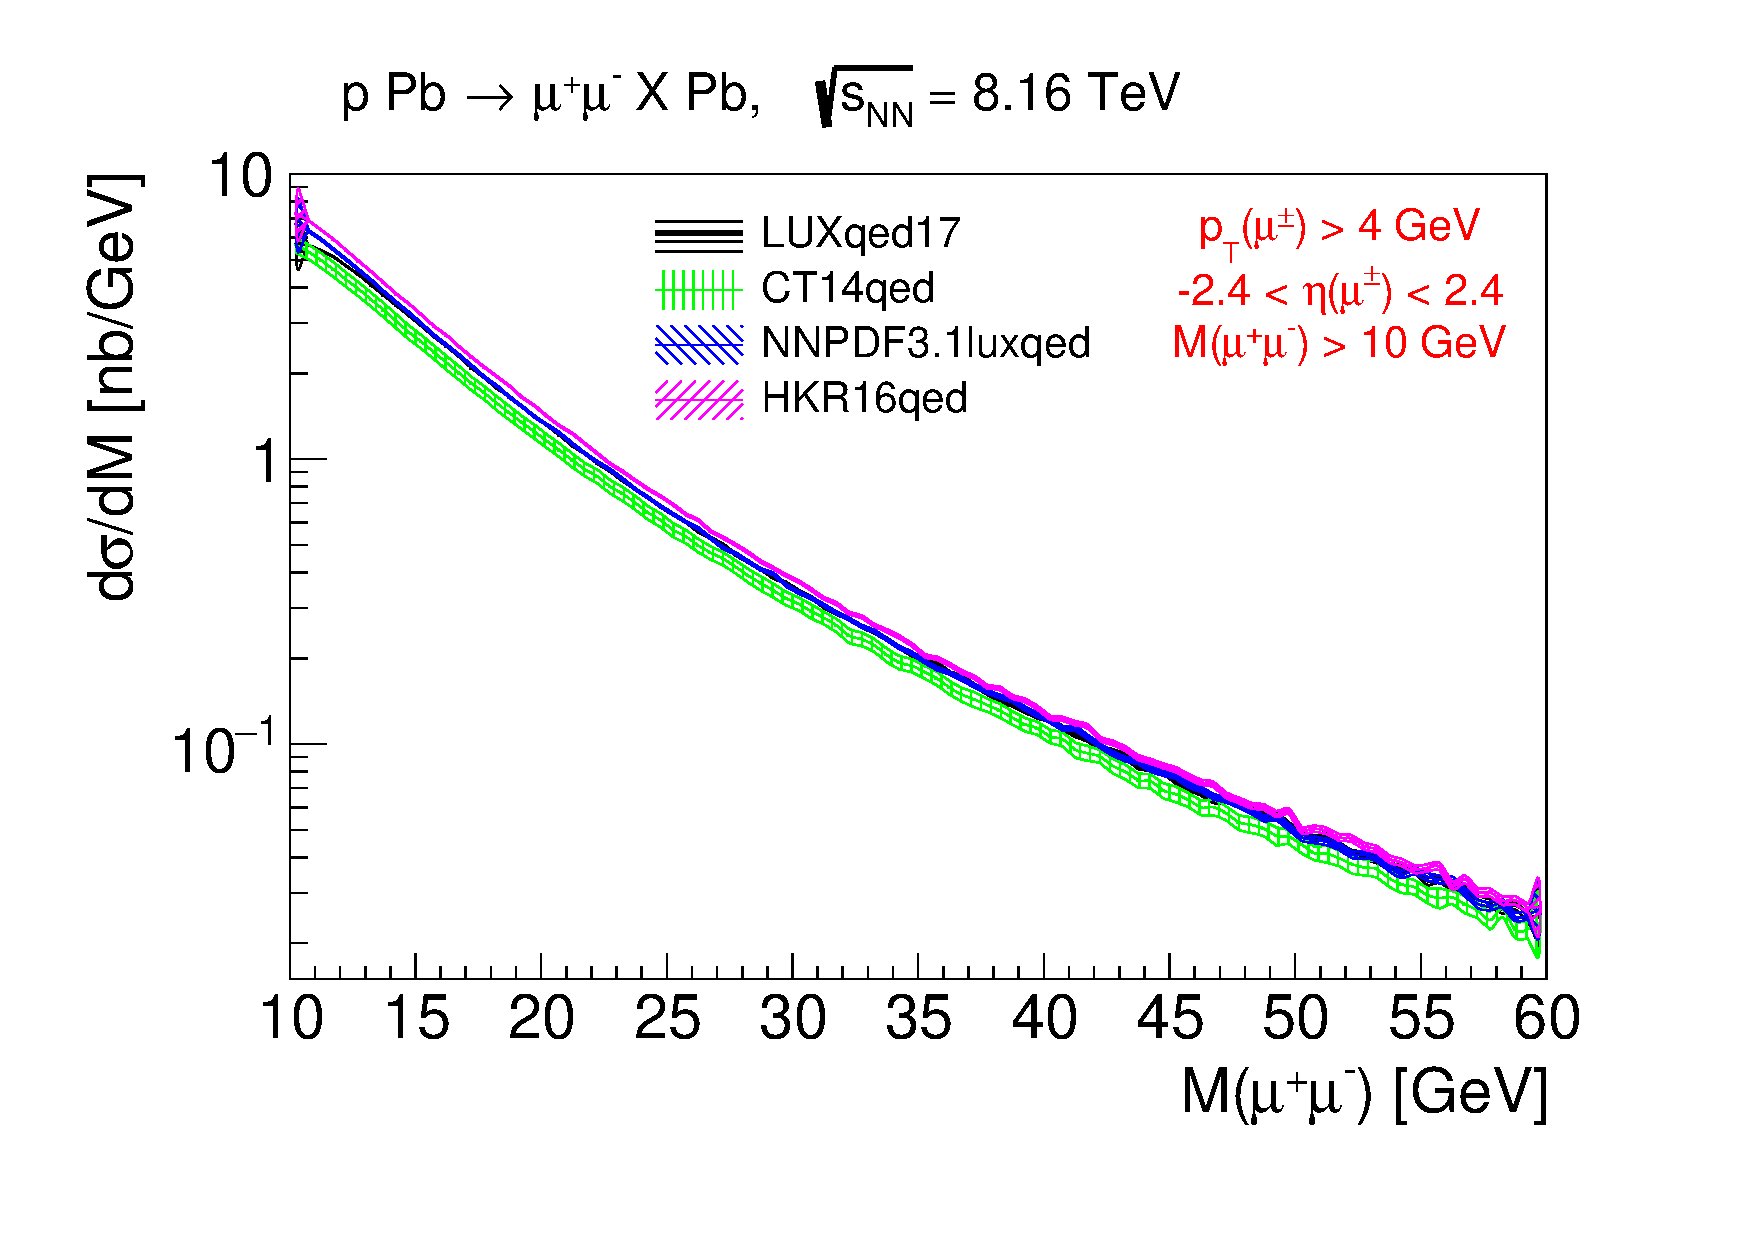
\includegraphics[width=0.4\textwidth]{figures/Mll_inc_cut.pdf}
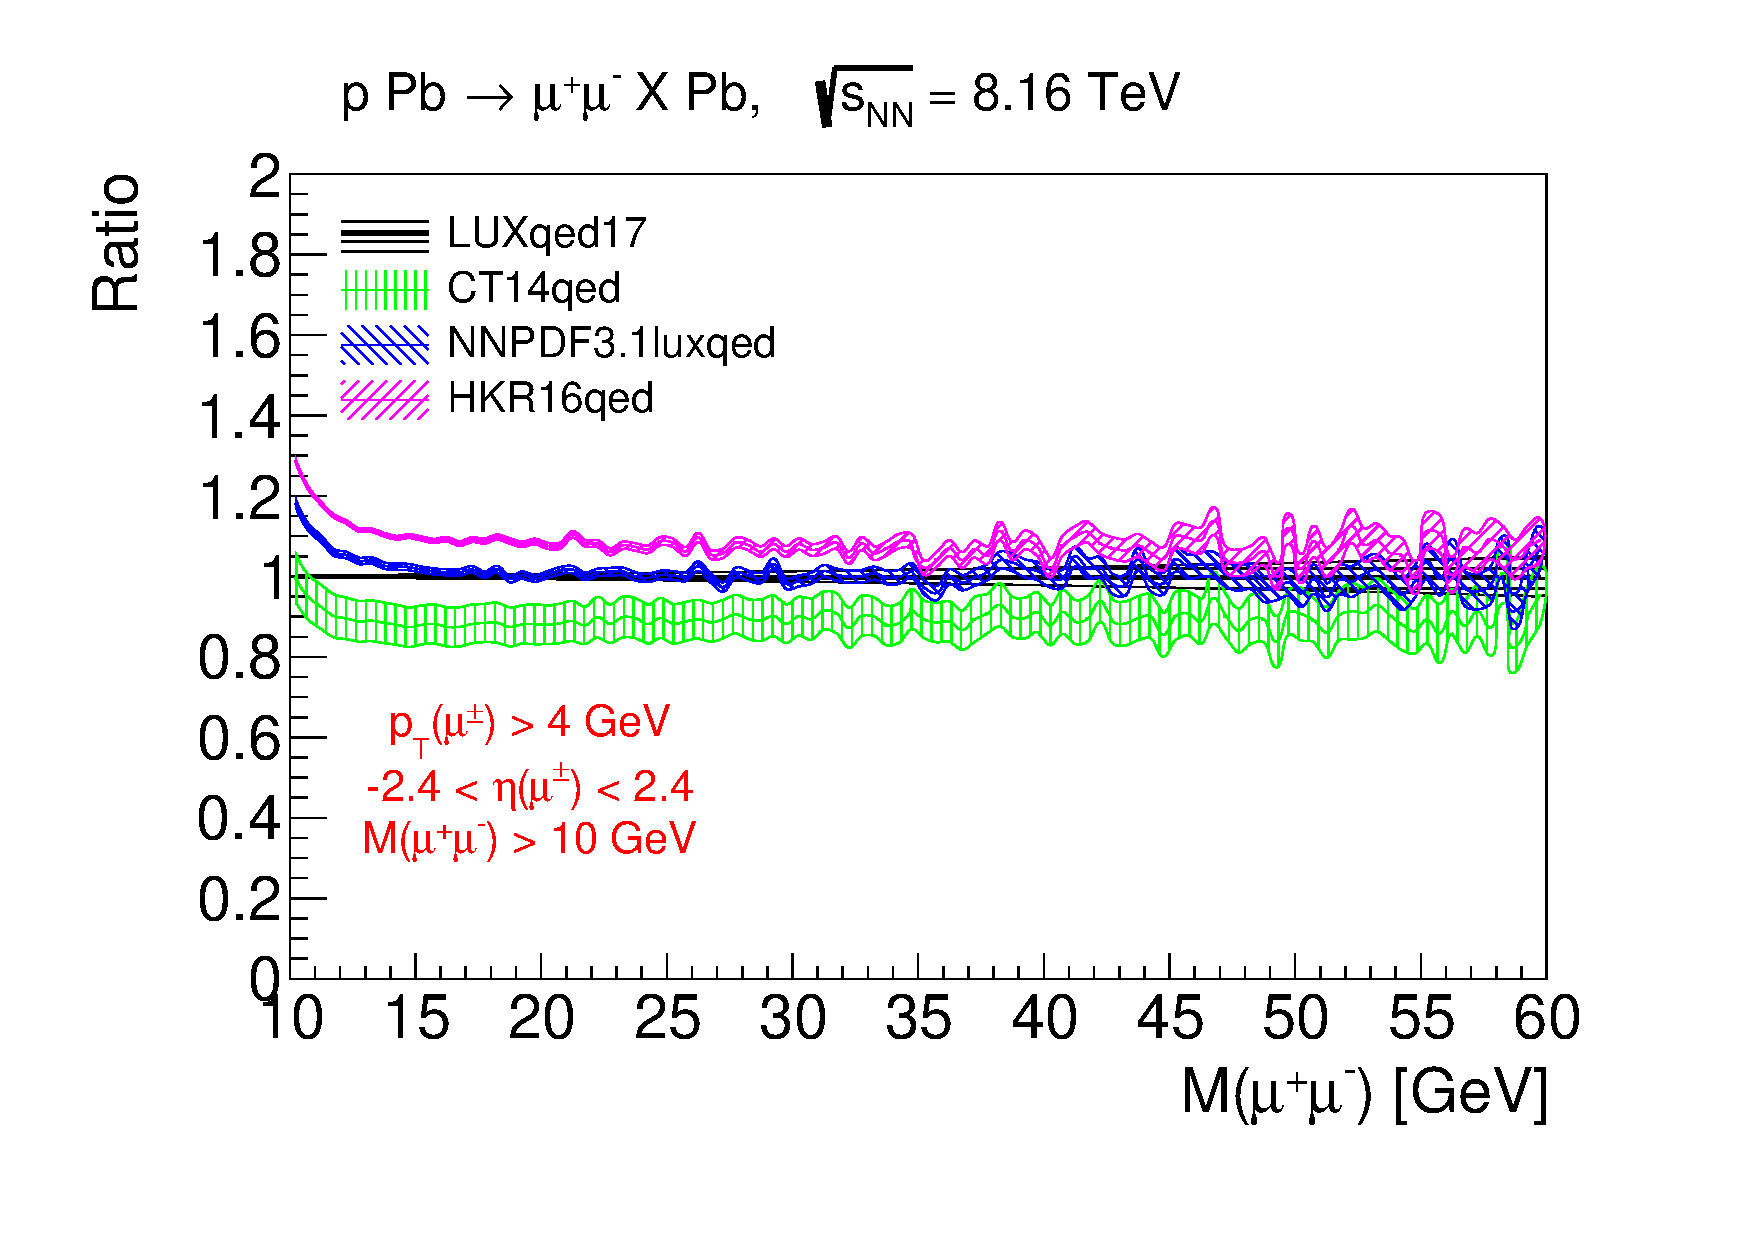
\includegraphics[width=0.4\textwidth]{figures/RatioMll_inc_cut.pdf}
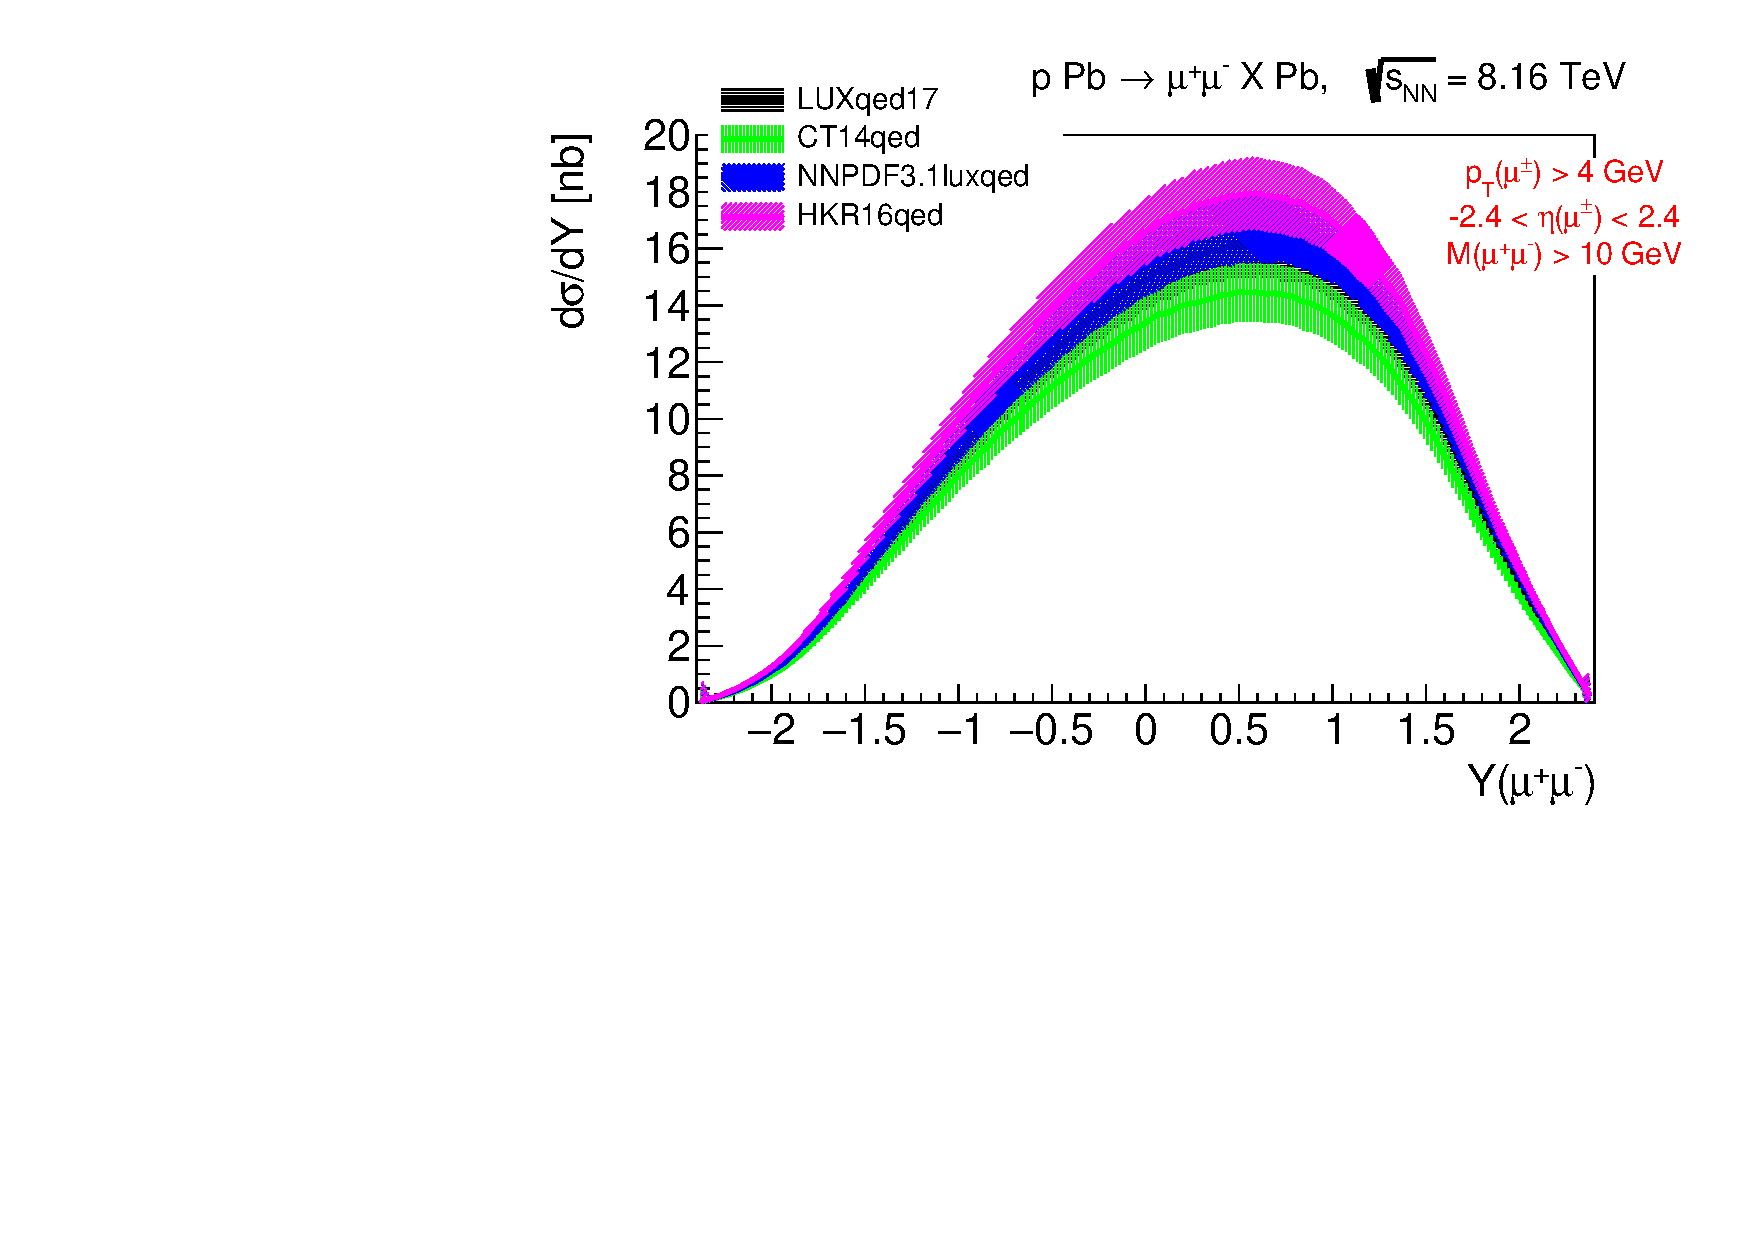
\includegraphics[width=0.4\textwidth]{figures/Yll_inc_cut.pdf}
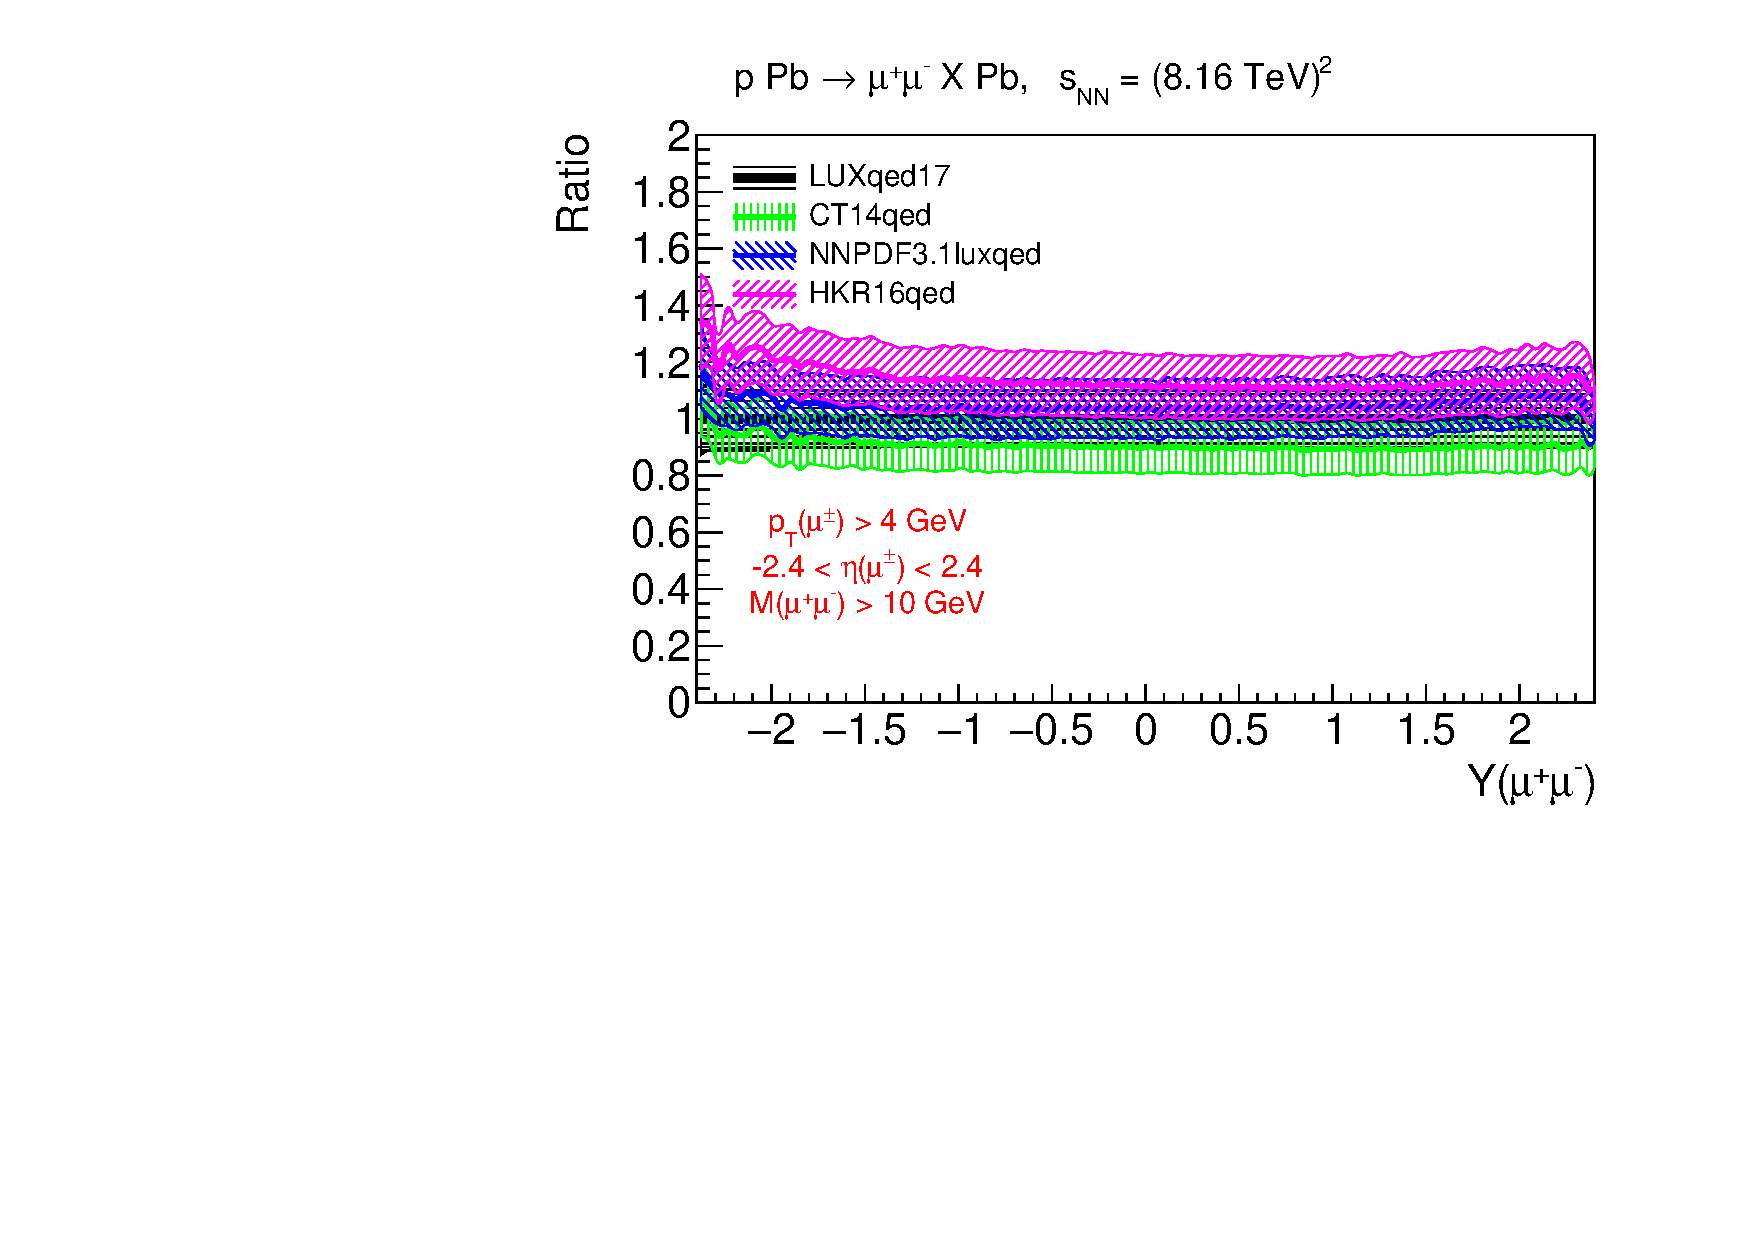
\includegraphics[width=0.4\textwidth]{figures/RatioYll_inc_cut.pdf}
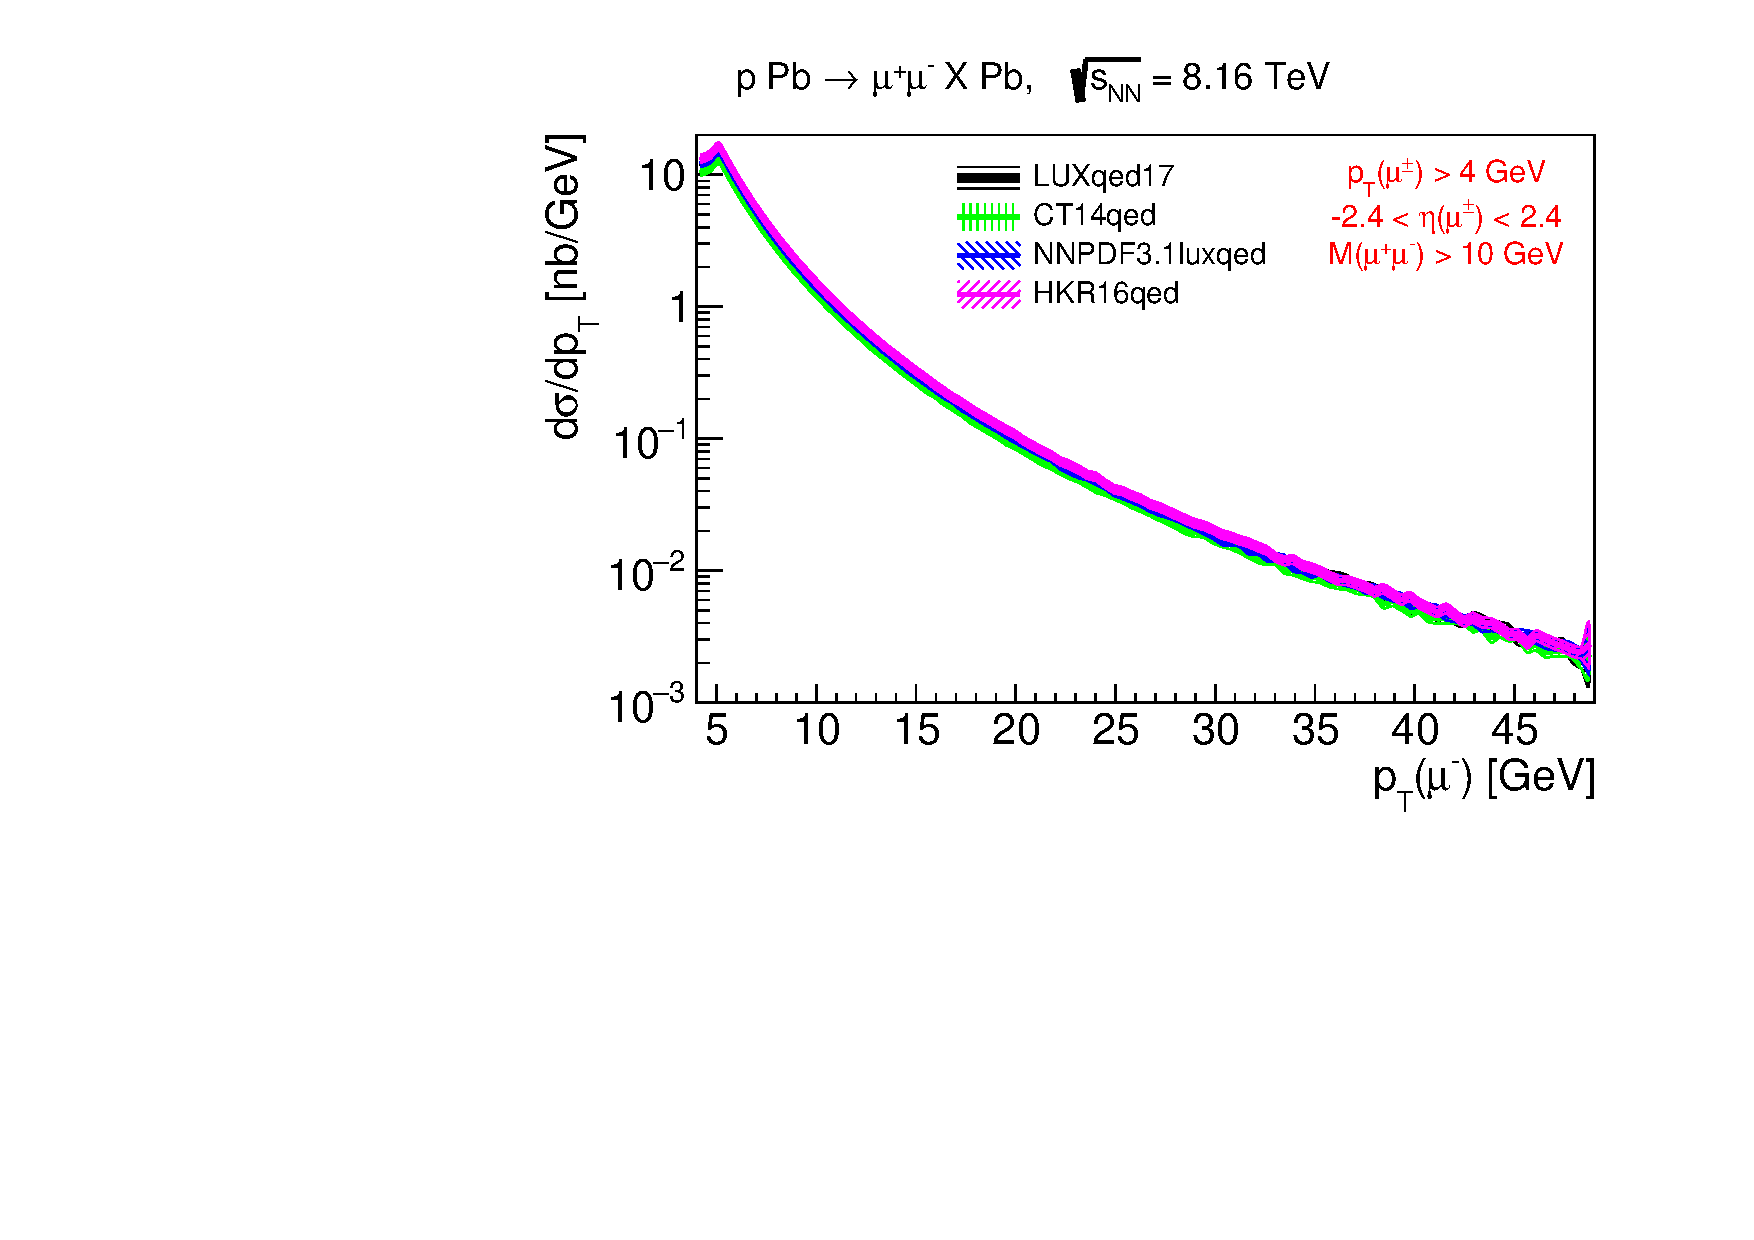
\includegraphics[width=0.4\textwidth]{figures/pTl_inc_cut.pdf}
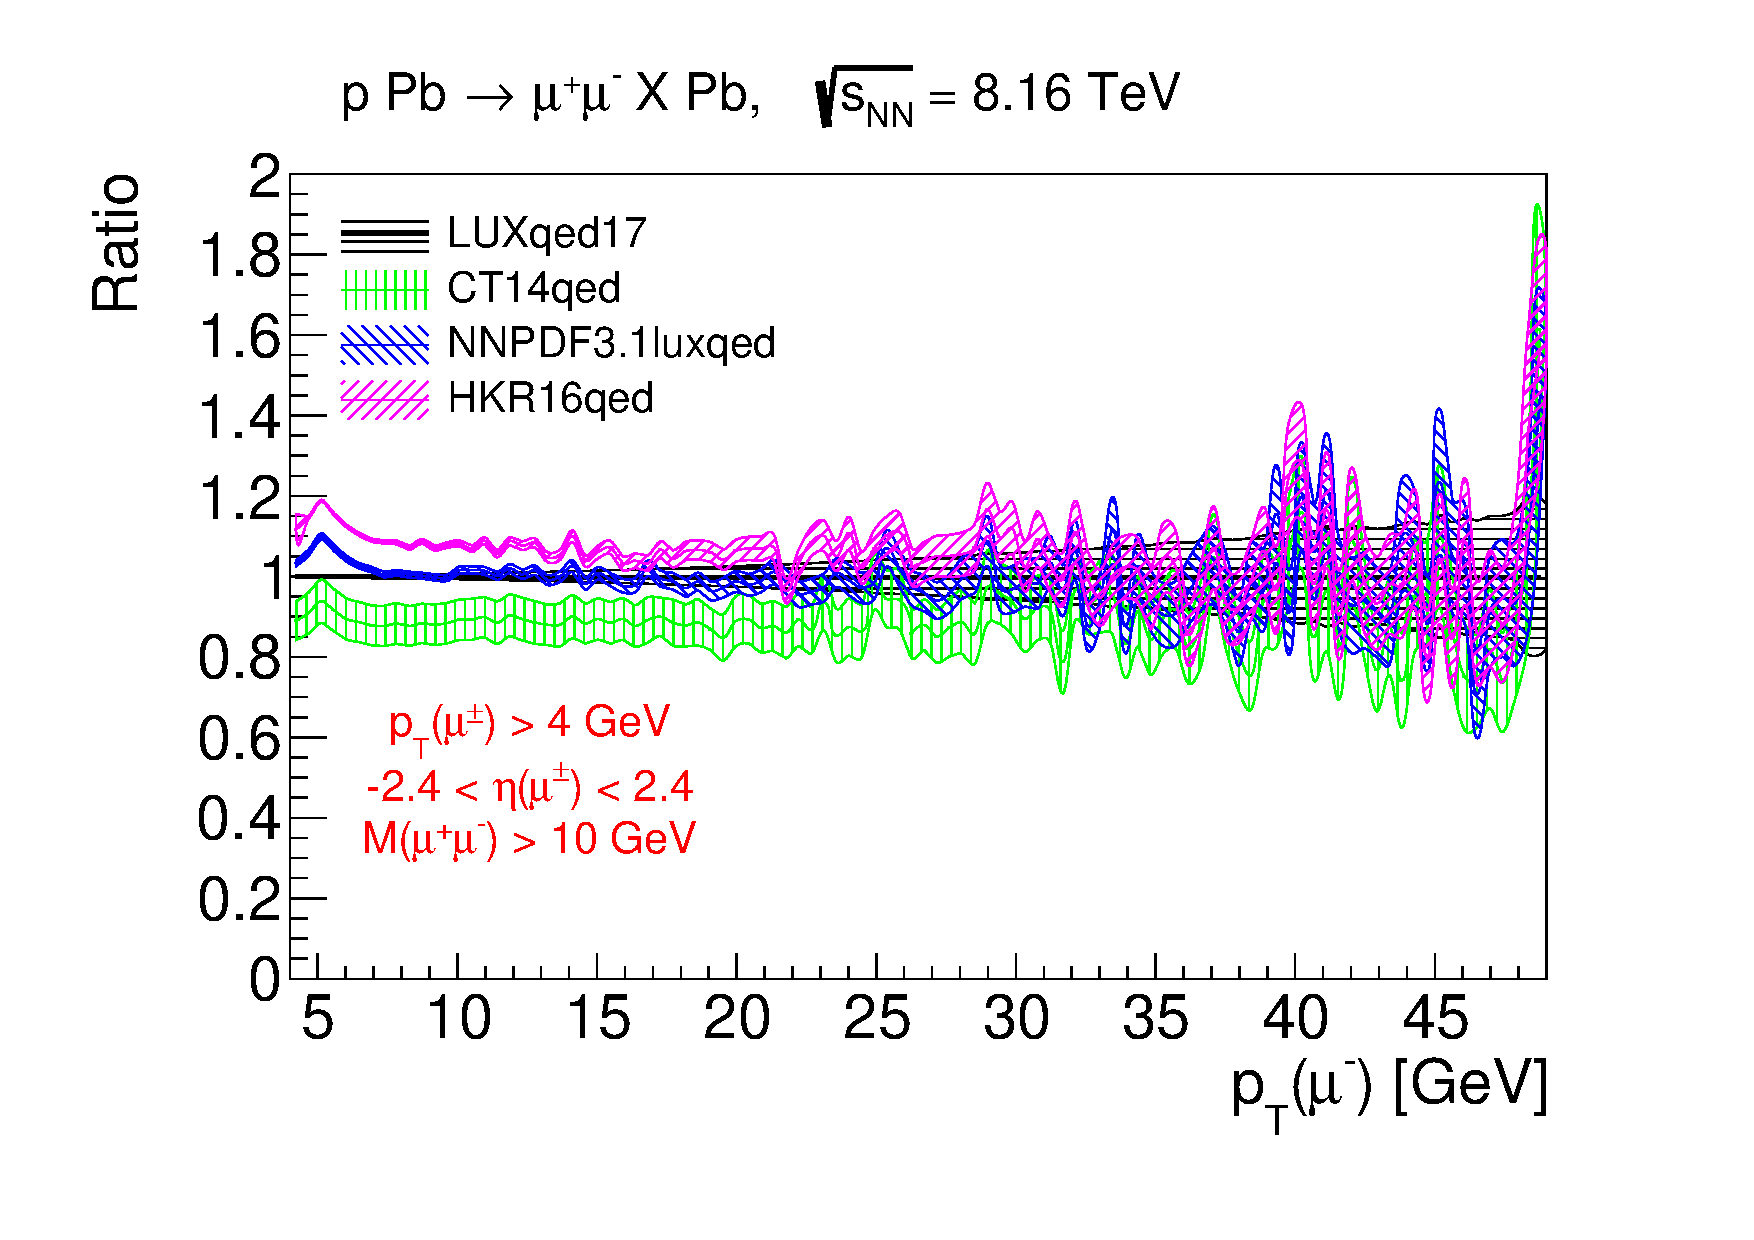
\includegraphics[width=0.4\textwidth]{figures/RatiopTl_inc_cut.pdf}
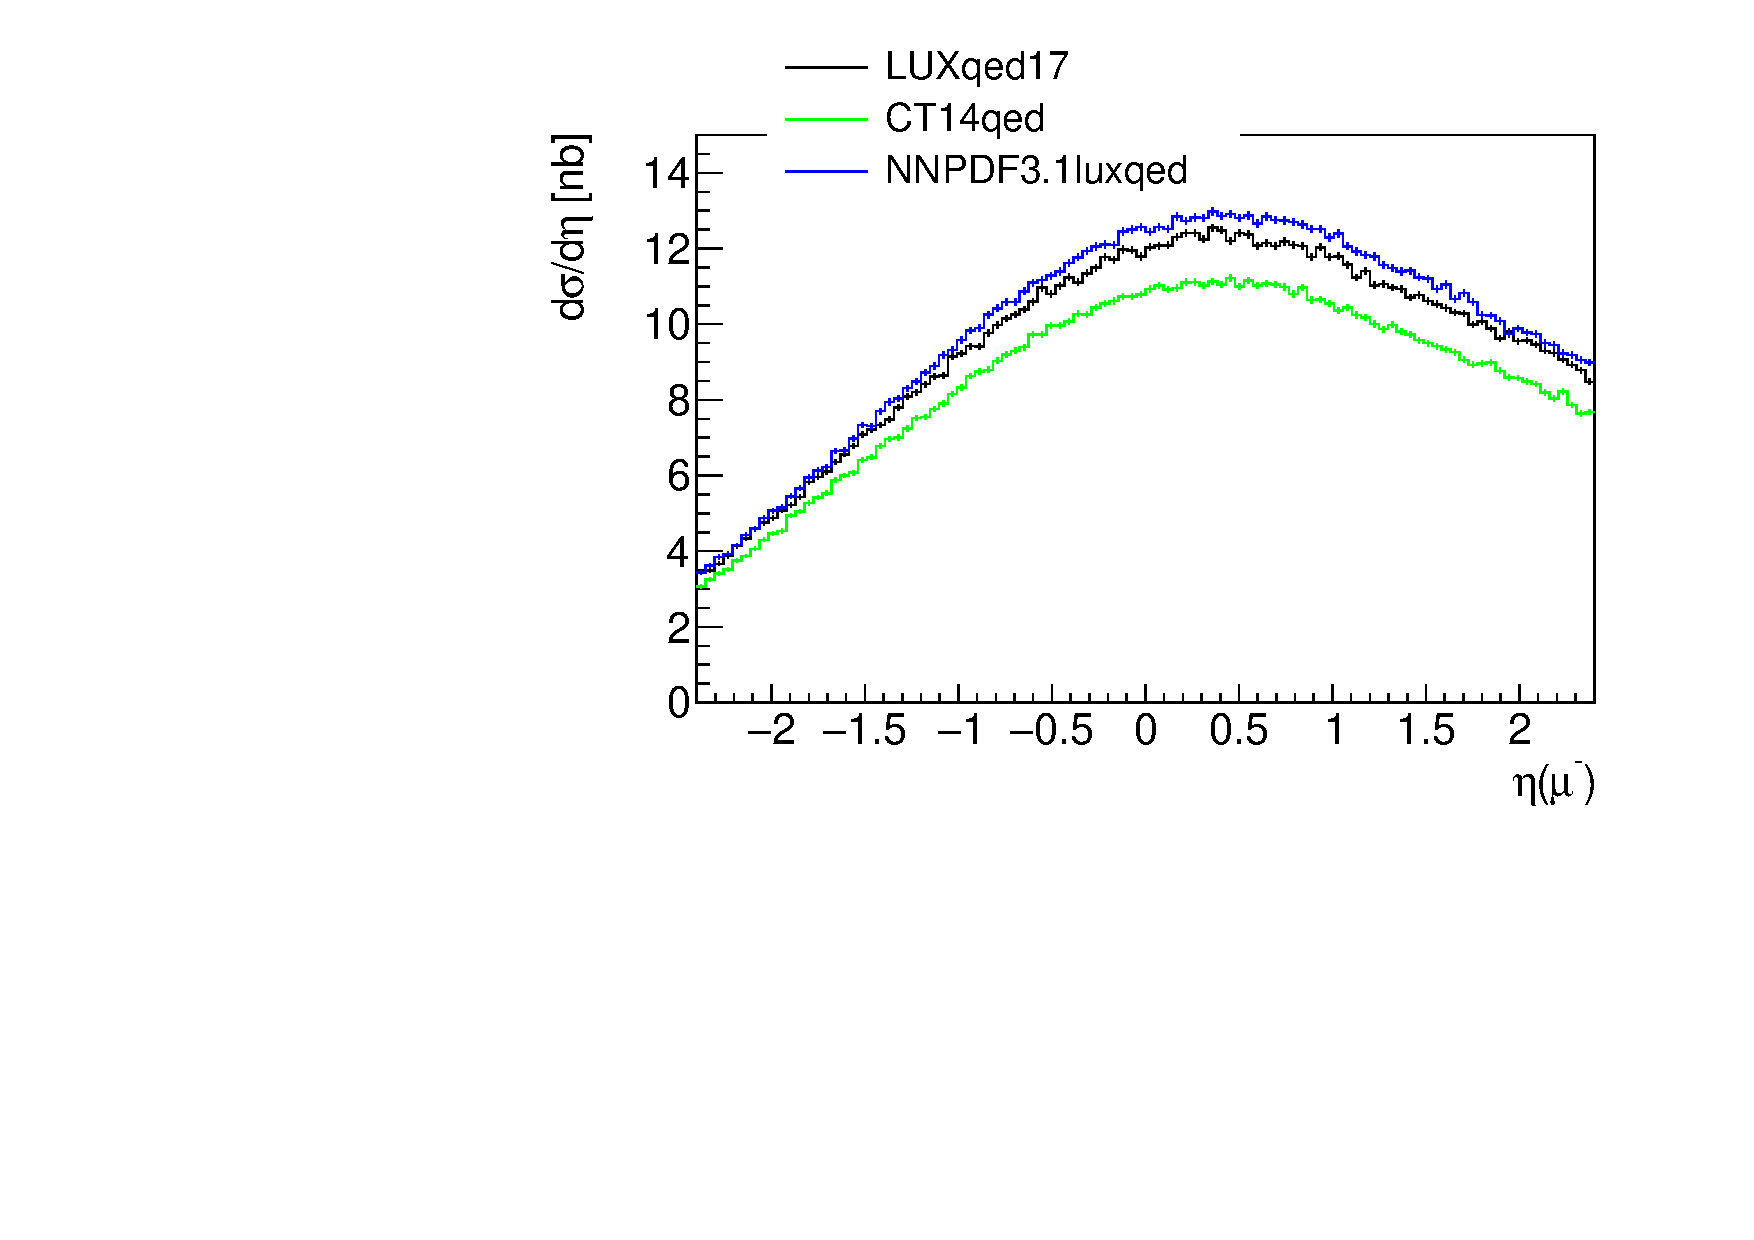
\includegraphics[width=0.4\textwidth]{figures/etal_inc_cut.pdf}
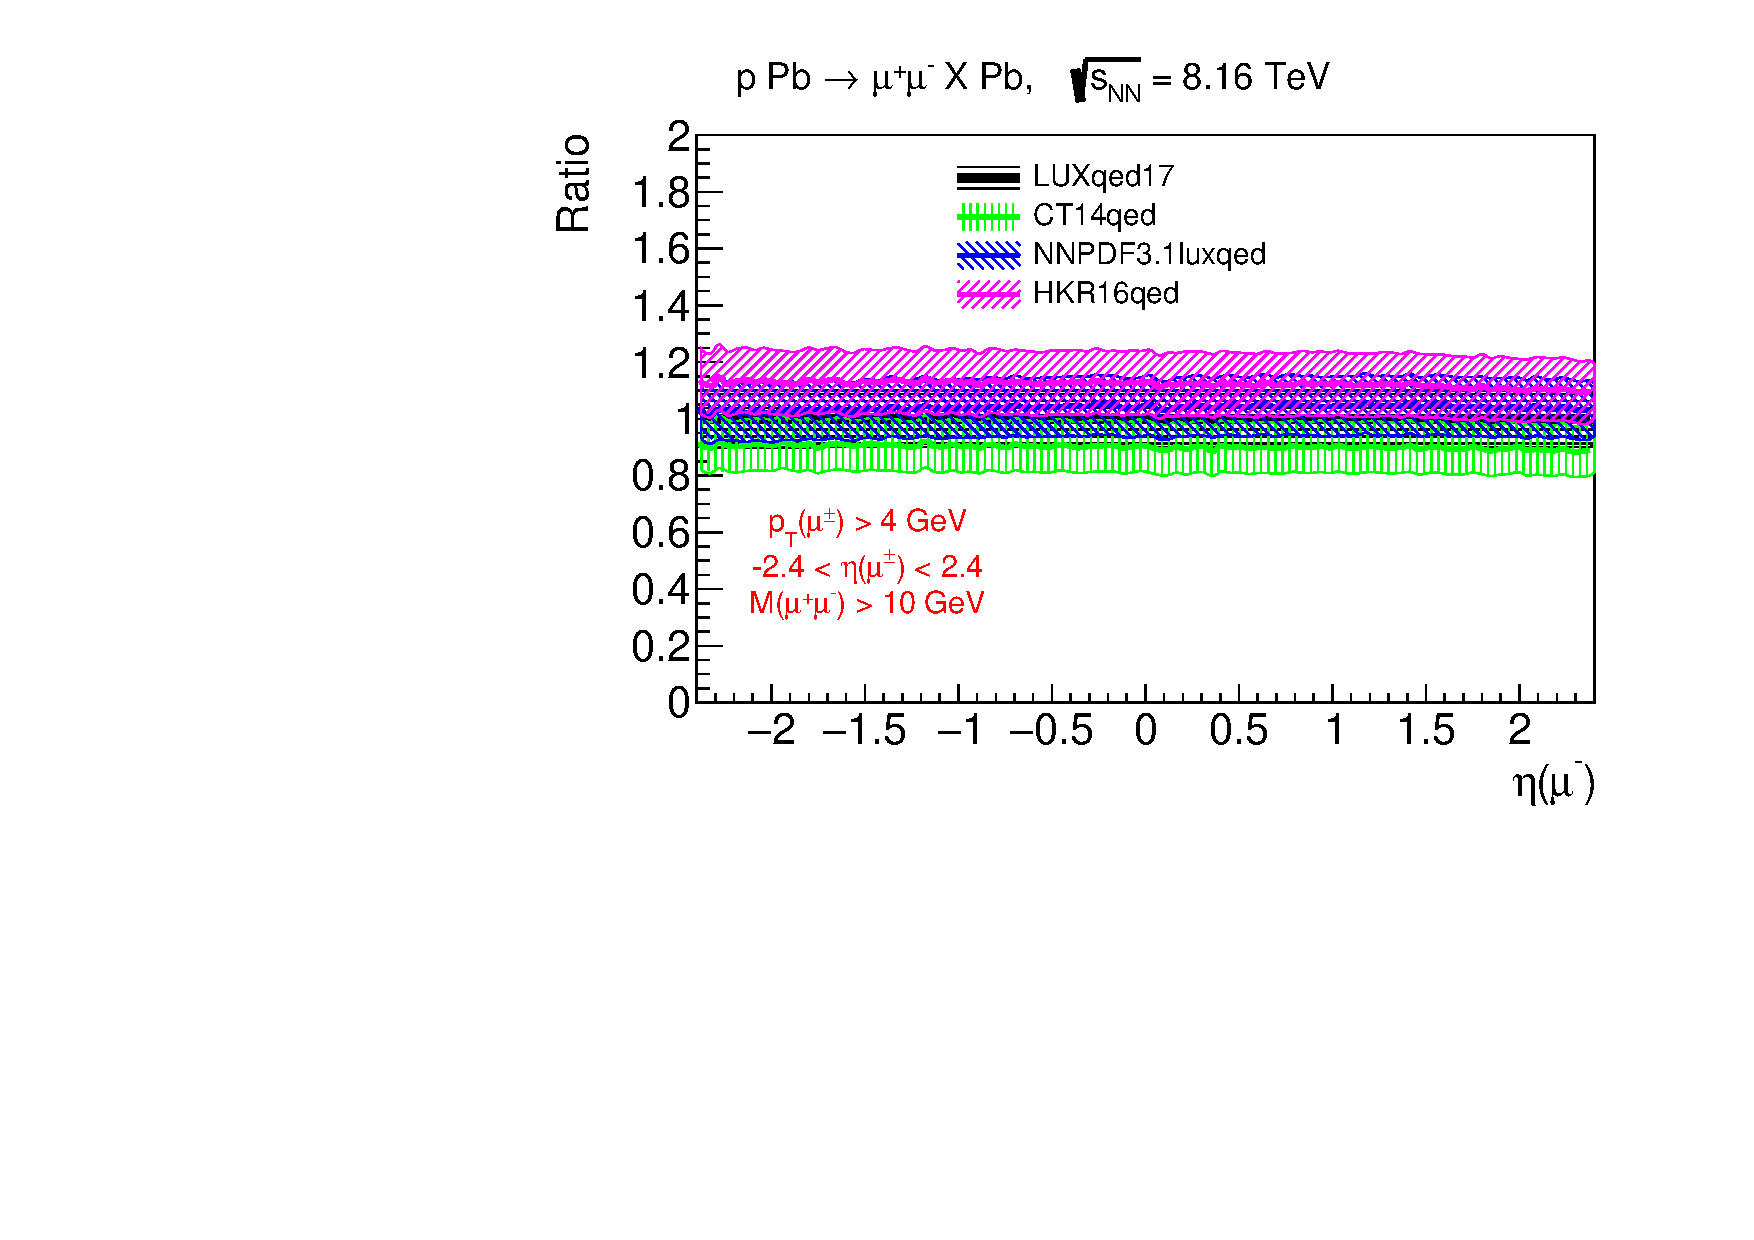
\includegraphics[width=0.4\textwidth]{figures/Ratioetal_inc_cut.pdf}
\caption{Inclusive distributions (fiducial regoin)}
\label{fig:inc_cut}
\end{figure}

The integrated fiducial cross-sections are summarized in Tab.~\ref{}.

(some discussion here...)

It should be made clear, that the calculations with collinear photons (at lowest order) produce leptons that are back-to-back in transverse kinematics. Therefore, to take the effect of inelastic photon virtuality into account, a dedicated parton shower algorithm should be used.

(mention we don't want to do extra PS; we would rather stick to kt factorization)
